% !TEX encoding = UTF-8 Unicode
\documentclass[a4paper, german, 12pt, onecolumn, oneside,bibliography=totoc,listof=totoc]{article}

\usepackage[utf8]{inputenc}
\usepackage[T1]{fontenc}
\usepackage[pdftex]{graphicx} % Einbindung von Grafiken (pdf, png, jpg)
\usepackage{float}            % bietet Option [H] für bombenfestes Verankern
\usepackage{wrapfig}
\usepackage{rotating}
\newcommand{\sturz}[1]{\rotatebox{90}{\parbox{20mm}{\raggedright #1}}} 
\usepackage[ngerman]{babel}   % Silbentrennung nach der neuen deutschen Rechtschreibung, z.B.: Sys-tem
%\usepackage{amstext}         % für Klartext via \text{} in Formeln
\usepackage{color}						% http://en.wikibooks.org/wiki/LaTeX/Colors
\usepackage[small,bf]{caption} % http://radio.wihome.net/wiki/?article=LaTeX:captions
\usepackage{sidecap}
\usepackage{amsmath}
\usepackage{amsfonts}					% wird with \mathbb gebraucht
\usepackage[safe]{tipa}
\usepackage{subfig}
	% ftp://ftp.tex.ac.uk/tex-archive/macros/latex/contrib/listings/listings.pdf
\usepackage{listings}

\usepackage[pdftex,pagebackref=true]{hyperref}	% für "klickbare" Verlinkung im Dokument
\hypersetup{
    %bookmarks=true,        % show bookmarks bar?
    unicode=false,          % non-Latin characters in Acrobat’s bookmarks
    pdftoolbar=true,        % show Acrobat’s toolbar?
    pdfmenubar=true,        % show Acrobat’s menu?
    pdffitwindow=false,     % window fit to page when opened
    pdfstartview={FitH},    % fits the width of the page to the window
    pdftitle={Diplomarbeit - Skalierbare Item Recommendation in Big-Data und Suchindexen},    % title
    pdfauthor={Tolleiv Nietsch},     % author
    pdfsubject={},   % subject of the document
    pdfcreator={Tolleiv Nietsch},   % creator of the document
    pdfproducer={TU Chemnitz}, % producer of the document
    pdfkeywords={recommender,collective intelligence}, % list of keywords
    pdfnewwindow=true,      % links in new window
    colorlinks=true,       % false: boxed links; true: colored links
    linkcolor=black,          % color of internal links
    citecolor=black,        % color of links to bibliography
    filecolor=black,      % color of file links
    urlcolor=black           % color of external links
}

\usepackage[square]{natbib}
\bibliographystyle{natdin}
%\usepackage[natbib=true,citecounter=true]{biblatex}
%\addbibresource{Literatur.bib}
%\bibpunct{(}{)}{;}{a}{,}{,}

\usepackage{multicol}

\usepackage[printonlyused]{acronym}
\renewcommand{\bflabel}[1]{\normalfont{\normalsize{#1}}\hfill}

\usepackage{parskip}          % zw. Absätzen: eine knappe Leerzeile statt hängender Einzüge
\usepackage{makeidx}          % Package zur Indexerstellung
\usepackage[colorinlistoftodos,textsize=tiny]{todonotes}	% bringt den todo befehl mit - "disable" in die Optionen zum ausschalten

\def\argmax{\operatorname*{arg\,max}}
\def\argmin{\operatorname*{arg\,min}}

\newenvironment{packed_enumerate}{
\begin{enumerate}
  \setlength{\itemsep}{1pt}
  \setlength{\parskip}{0pt}
  \setlength{\parsep}{0pt}}{\end{enumerate}
}

\renewcommand{\figurename}{Abb.}
%%%%%%%%%%%%%%%%%%%%%%%%%%%%%%%%%%%%%%%%%%%%%%%%%%%%%%%%%%%%%%%%%%%%%%%%%%%%%%
%
% Größenanpassungen
%
\setlength{\unitlength}{1cm}
\setlength{\oddsidemargin}{0cm}
\setlength{\evensidemargin}{0cm}
\setlength{\textwidth}{16.1cm}
\setlength{\topmargin}{-1.2cm}
\setlength{\textheight}{23cm}
\columnsep 0.5cm
%
%%%%%%%%%%%%%%%%%%%%%%%%%%%%%%%%%%%%%%%%%%%%%%%%%%%%%%%%%%%%%%%%%%%%%%%%%%%%%%
\newcommand{\addtoindex}[1]{#1\index{#1}}
\newcommand{\nosubsubsection}[1] {{\textit{#1}}\newline}
\newcommand{\footnoteremember}[2]{
  \footnote{#2}
  \newcounter{#1}
  \setcounter{#1}{\value{footnote}}
} \newcommand{\footnoterecall}[1]{
  \footnotemark[\value{#1}]
} 

\sloppy                       % großzügiger Zeilenumbruch 
\makeindex 

\hyphenation{Grund-elemente}	% definierte Silbentrennung
\hyphenation{Daten-menge}
\hyphenation{Werbe-banner}

\begin{document}
\lstset{basicstyle=\linespread{1}\scriptsize\ttfamily, basewidth=0.51em}

\pagenumbering{roman}
\pagestyle{empty}
\begin{titlepage}
\begin{figure}
  \begin{center}
    \hbox to \hsize{%
      \begin{tabular}[m]{c}
        
\includegraphics[width=2.5cm]{Abbildungen/tuc_medieninfo_logo.jpg}
      \end{tabular}
      \hfill%
      \begin{tabular}[m]{c}
        Technische Universität Chemnitz \\
        Fakultät für Informatik \\
        Professur Künstliche Intelligenz \\
      \end{tabular}%
    }
  \end{center}
\end{figure}

\begin{center}
\rule{0pt}{0pt}
\vfill
\vfill

\includegraphics[width=8cm]{Abbildungen/TUC_deutsch_SW.pdf}
\vfill
\vfill
\vfill
\vfill

\begin{Huge}
Diplomarbeit \\
\end{Huge}
im Studiengang Angewandte Informatik \\
~\\
\begin{footnotesize}
Vorgelegt von \\
\end{footnotesize}
\begin{large}
Tolleiv Nietsch \\
\end{large}
\begin{footnotesize}
--- \\
\end{footnotesize}

\vfill
\vfill

\begin{large}Skalierbare Item Recommendation in Big-Data und Suchindexen\end{large} \\

%~ \\
%\hrule
%\begin{Large}Subtitle\end{Large}

\vfill

\end{center}
\end{titlepage}

\newpage
~
\newpage

~
\vspace{5cm}


\begin{large}
\textbf{Selbstständigkeitserklärung} \\ \\
\end{large}
Hiermit erkläre ich, dass ich die vorliegende schriftliche Arbeit selbstständig und ohne Benutzung anderer als der angegebenen Quellen und Hilfsmittel angefertigt habe. \\
Die vorliegende Arbeit ist frei von Plagiaten. Alle Ausführungen, die wörtlich oder inhaltlich aus anderen Schriften entnommen sind, habe ich als solche kenntlich gemacht. \\
Diese Arbeit wurde in gleicher oder ähnlicher Form noch bei keinem anderen Prüfer als Prüfungsleistung eingereicht und ist auch noch nicht veröffentlicht.\\

\vfill
\begin{tabular*}{0.5\textwidth}{@{\extracolsep{\fill}}ll}
Vorname: & Tolleiv \\
Name: & Nietsch \\
Matrikelnummer: & 172314 \\
\end{tabular*}

\vfill
\vfill

Chemnitz, den 29.03.2012 \\
\medskip
\medskip

\underline{~~~~~~~~~~~~~~~~~~~~~~~~~~~~~~~~~~~~~~~~}\\
Tolleiv Nietsch\\


\vfill
\begin{large}
\textbf{Betreuung und Prüfung durch:} \\ \\
\end{large}
\begin{tabular*}{\textwidth}{@{\extracolsep{\fill}}ll}
Prof. Dr. Fred Hamker, & Professur Künstliche Intelligenz, TU-Chemnitz \\
Dr. Johannes Steinmüller & Professur Künstliche Intelligenz, TU-Chemnitz \\ 
\end{tabular*}

\begin{footnotesize}
Technische Universität Chemnitz, Fakultät für Informatik \\
Straße der Nationen 62, 09107 Chemnitz
\end{footnotesize}

\newpage

					% und eidesstattliche Erklärung

~
\vspace{5cm}

\begin{large}
\textbf{Kurzfassung} \\ \\
\end{large}
tbw

\newpage
\setcounter{page}{1}					% Seitenzahl zurück	
\tableofcontents					% Inhaltsverz.
\newpage

\listoftodos \newpage

\pagenumbering{arabic}
\pagestyle{plain} 
\renewcommand{\baselinestretch}{1.50}\normalsize
\setcounter{page}{1}					% Seitenzahl zurück	

%%%%%%%%%%%%%%%%%%%%%%%%%%%%%%%%%%%%%%%%%%%%%%%%%%%%%%%%%%%%%%%%%%%%%%%%

\section{Einleitung}


Hinweis das ``Elemente'' und ``Item'' oft als Synonym verwendet werden, ähnlich wie auch ``Rating'' und ``Bewertung'' gleichzusetzen sind.

Goldberg92 -> Ursprung des Ausdrucks

Ggf. direkt Terminologie ergänzen - gutes Beispiel Goldberg01 (Kap 3.1)

QVC Italia als Usecase vorstellen und einordnen

\todo[color=red]{Hindernis}
\todo[color=orange]{Wichtige Aufgabe}
\todo[color=yellow]{Aufgabe abhängig von anderen}
\todo[color=green]{Mögliche Ergänzung / weitere Anregung}
\todo[color=white]{}\newpage
\section{Grundlagen}

Im folgenden Abschnitt werden die notwendigen Grundlagen der verschiedenen Bestandteile einer personalisierten Suche beschrieben. Der erste Abschnitt beschreibt den Aufbau von Suchindexen und die Möglichkeiten zur Personalisierung der Ergebnisse. Der darauf folgende Abschnitt fasst Konzepte zur Bildung von Empfehlungen zusammen. Abschnitt \ref{sec:filtermethods} greift die Methode des kollaborativen Filterns nochmals auf und beschreibt die zugrunde liegenden Rechenmodelle. Der darauf folgende Abschied \ref{sec:filterissues} beschreibt Herausforderungen die sich im praktischen Umgang mit kollaborativen Filtermodellen ergeben. 

%	Auf welchen Themen und Techniken baut die Arbeit auf.
\todo{Formulierung kontrollieren}

\subsection{Suchindexe}
\label{sec:search}

Mit dem Begriffen ``Suche'' und ``Suchmaschinen'' werden umgangssprachlich zahlreiche Methoden des  \ac{IR} beschrieben, die durch Internet-Dienste wie Google\footnote{http://www.google.com} im Alltag vieler Menschen präsent sind. Im \acs{IR} wird eine ``Suche'' formal als die Extraktion von Informationen aus einer Menge unstrukturierter Daten definiert. Innerhalb eines \acs{IR} Systems liegen die Daten in Form von \textit{Dokumenten} (Texte, Bilder, Videos) vor. Bei der Benutzung des \acs{IR} Systems formuliert der Nutzer seinen \textit{Informationsbedarf} mit Hilfe von \textit{Anfragen}. Dokumente werden als \textit{relevant} bezeichnet, wenn die darin enthaltene Information dem Bedarf des Nutzers genügt. Im weiteren Sinne umfasst \acs{IR} zudem das Filtern, Klassifizieren und Verarbeiten der gefundenen Dokumente.  \citep{Manning2008}

Die durch den Nutzer formulierten Anfragen sind dabei, im Gegensatz zu Anfragen an strukturierte Datenbanken, nicht zwingend eindeutig. Sucht der Nutzer etwa nach ``Fantasy Buch'', kann ``Harry Potter'' in den Augen des Nutzers ein relevantes Dokument sein, ohne dass die Begriffe ``Fantasy'' oder ``Buch'' explizit darin vorkommen.%http://nlp.stanford.edu/IR-book/pdf/04const.pdf

\subsubsection{Indexbildung} \label{sec:indexcreation}

Da es bei einer großen Anzahl von vorhandenen Dokumenten sehr ineffizient wäre, wenn bei jeder Anfrage jedes Dokument geprüft werden müsste, wird eine \textit{invertierten Index} verwendet um Informationen zu Dokumenten abzubilden. Die Indexierung erfolgt dabei in vier Schritten, welche für zwei Beispieldokumente\footnote{Ausschnitte aus ``Julius Caesar'' von William Shakespeare} wie folgt verlaufen:

\begin{enumerate}
\item Sammeln aller Dokumente und Zuordnung von eindeutigen Bezeichnern (\textit{docID}) \\ { \scriptsize ..., 20:\fbox{Friends, Romans, countrymen}, 21:\fbox{So let it be with Caesar.},... }
\item Extraktion der Dokumentenmerkmale (z.B. Wörter) \\ { \scriptsize \fbox{Friends} \fbox{Romans} \fbox{countrymen} \fbox{Caesar} }
\item Normalisierung der Merkmale (z.B. Reduzierung auf Wortstämme) \\ { \scriptsize \fbox{friend} \fbox{roman} \fbox{countryman} \fbox{caesar} }
\item Indexbildung, Zuordnung der \textit{docID} zu den Einträgen der sortierten Merkmalsliste
{ \scriptsize \begin{tabular}[b]{lcl}
 \fbox{caesar} & $\longmapsto$ & \fbox{ 21 } \\
 \fbox{countryman} & $\longmapsto$ & \fbox{ 11 }\fbox{ 20 } \\
 \fbox{friend} & $\longmapsto$& \fbox{ 15 }\fbox{ 20 }\fbox{ 73 }\\
 \fbox{roman}& $\longmapsto$ & \fbox{ 20 }\fbox{ 32 }\\ 
 ... & &
\end{tabular} }
\end{enumerate}

Die in den Schritten 1 bis 3 durchgeführten Verarbeitungsschritte sind immer abhängig von dem gegebenen Kontext. Entspricht z.B. im herkömmlichen Verständnis jede Datei einem Dokument, so muss bei der Verarbeitung des MBox-Formates\footnote{siehe RFC 4155 - http://tools.ietf.org/rfc/rfc4155.txt} jede Zeile einer Datei als einzelnes Dokument gesehen werden. Auch die Wahl einer geeigneten Methode zur Wortstammbildung (auch ``Stemming'') und das Filtern von nicht relevanten Wörtern mit Hilfe sog. ``Stopwörter'' hängt vom gegebenen Kontext ab. \citep[Kap. 2]{Manning2008}. 

Formuliert der Nutzer nun seine Anfrage, durchläuft diese ebenfalls die Schritte 2 und 3 bevor Dokumente mit Hilfe des Index gefunden werden können. Besteht die Anfrage aus mehreren Bestandteilen, wird die Liste der relevanten Dokumente aus der Schnittmenge der für die einzelnen Teile gefundenen Dokumentenmengen gebildet. Ergänzend existieren verschiedene Erweiterungen des invertierten Index. Diese ermöglichen beispielsweise noch effizienter in sehr großen Dokumentenbeständen suchen zu können, die Position der Merkmale innerhalb des Dokumentes nutzbar zu machen oder den Umfang des Index einzuschränken. Sie werden u.a. in \citep[Kap. 3,4,5]{Manning2008} beschrieben und hier zur Wahrung des Umfangs ausgelassen.

\subsubsection{Relevanzberechnung}\label{sec:searchrelevance}\label{tfidf}
Die reine Generierung einer Dokumentenliste als Ergebnis der Anfrage genügt vor allem bei großen Dokumentenbeständen nicht. Mögliche Methoden, um die Listen  entsprechend der Relevanz eines Dokumentes zu sortieren, sind zum einen das \textit{Tf-idf Maß} und bei untereinander verknüpften Dokumenten der \textit{PageRank}.

\paragraph{Tf-idf Maß} Zur Bildung dieses Maßes wird die Relevanz des Terms $i$ innerhalb des Dokumentes $d$ und die Relevanz des Terms innerhalb des gesamten Dokumentenbestands ins Verhältnis gesetzt.
\begin{align}
\text{tf}(i, d) & = \frac{\text{freq}(i, d)}{\text{max}_{z \in Z}(\text{freq}(z, d))} \\
\text{idf}(i) & = \log{\frac{N}{n(i)}} \\
\text{tf-idf}(i, d) & = \text{tf}(i ,d) \ast \text{idf}(i) \label{form:tfidf}
\end{align}

Um die Relevanz eines Terms bezüglich eines Dokumentes abzubilden, wird die relative Häufigkeit mit der der Term innerhalb des Dokumentes vorkommt, genutzt. Die sog. \textit{Termfrequenz} bildet sich entsprechend aus dem Verhältnis der Anzahl der Vorkommen des Terms innerhalb des Dokumentes ($freq(i,j)$) zur maximalen Anzahl aller anderen Terme $Z$ im Dokument. Mit Hilfe der inversen Dokumentenfrequenz (\acs{IDF}) wird die \acf{TF} eines Terms abgewertet, wenn dieser in nahezu jedem Dokument vorkommt und aufgewertet, wenn er nur selten genutzt wird. Die \acs{IDF} wird aus dem Verhältnis der Gesamtdokumentenzahl $N$ zur Anzahl der Dokumente die den Term $i$ enthalten ($n(i)$), gebildet.

Das \textit{tf-idf Maß} bildet sich entsprechend Formel (\ref{form:tfidf}) aus dem Produkt der beiden Teilmaße und ist:
\begin{itemize}
\item hoch: wenn der Term $i$ oft in einer kleinen Anzahl von Dokumenten vorkommt und sich gut zur Unterscheidung von Dokumenten eignet
\item niedrig: wenn der Term selten im Dokument vorkommt oder in vielen verschiedenen Dokumenten genutzt wird
\item minimal: wenn der Term in nahezu jedem Dokument vorkommt
\end{itemize}

Die Summe der Relevanz eines Dokuments bezüglich aller Teilterme der Anfrage $q$ bildet dann die Grundlage, um die erzeugte Dokumentenliste zu sortieren.\citep{Manning2008} 
\begin{align}
\text{score}(q,d) & = \sum_{t \in q}{\text{tf-idf}(t,d)}  \label{form:docscore}
\end{align}

\paragraph{PageRank} Sind die Dokumente untereinander verknüpft, kann man auch die Popularität eines Dokumentes zur Grundlage der Anordnung in der Ergebnisliste machen. Diese Popularität wird i.d.R. in Form des PageRank ausgedrückt. Dieser korreliert mit der Wahrscheinlichkeit, dass ein zufällig über den Verknüpfungsgraphen laufender Nutzer ein bestimmtes Dokument erreicht. Dokumente, auf die häufig verwiesen wird, besitzen demnach einen hohe PageRank und Verweise von populären Dokumenten üben einen größeren Effekt auf den PageRank der verknüpften Dokumente aus.
\begin{align}
R(d) & = c \sum_{v \in B_d}{\frac{R(v)}{N_v}} + cE(d) \label{form:pagerank}
\end{align}

Berechnet wird der PageRank $R$ einer Seite $u$ mit Hilfe der Formel (\ref{form:pagerank}). Der Faktor $c < 1$ dient dabei zur Abstraktion des Verlustes durch Seiten ohne ausgehende Verweise. Der Vektor $E$ bildet die Wahrscheinlichkeit ab, dass der Nutzer seinen Pfad unterbricht und zufällig bei Dokument $d$ fortsetzt.\citep{pagerank,Manning2008}

\subsubsection{Personalisierung}\label{sec:personalresultstheorie}

Die Personalisierung der Dokumentenlisten kann über verschiedene Wege erreicht werden. Der offensichtliche ist, die der Anfrage entsprechende Dokumentenliste anhand der Präferenzen eines Nutzerprofils umzusortieren. Eine weitere Möglichkeit ist, die durch den Nutzer formulierte Anfrage vor der eigentlichen Verarbeitung mit Informationen des Nutzerprofils zu erweitern.

Die erste Methode wird zum Beispiel in \citep{Durao12} beschrieben. Um die Dokumentenliste zu personalisieren, wird zunächst ein schlagwortbasiertes Nutzerprofil aufgebaut, welches die bevorzugten Schlagworte $t \in T_u$ in Bezug auf verschiedene Faktoren $F$ und deren relative Frequenz $T_f \subset T_u$ beinhaltet. Die Gewichtung der Faktoren untereinander wird durch $\alpha_f$ realisiert. Zusätzlich werden auch zu jedem Dokument entsprechende Tags $T_d$ gepflegt, so dass die Ähnlichkeit von Nutzerprofil und Dokument mit Hilfe der Kosinus-Ähnlichkeitsmaßes (siehe Abschnitt \ref{sec:cossim}) berechnet werden kann. Da die initiale Dokumentenliste anhand des Tf-idf Maßes sortiert wird, ergibt sich die endgültige Bewertung für den Nutzer $u$ aus:  (vgl. \citep{Durao12})
\begin{align}
\text{score}(q,d,u) & = \text{score}_{\text{tf-idf}}(q,d) * \sum_{f \in |F|}{\alpha_f \frac{\overrightarrow{T_d} \overrightarrow{T_f}}{|\overrightarrow{T_d}| |\overrightarrow{T_f}|}} \label{form:personalresultstheorie}
\end{align}

Die Anpassung der Anfrage vor der Verarbeitung durch die Suche wird zum Beispiel in \citep{Boughareb11} genutzt. Das Nutzerprofil wird dabei aus der Liste aller vorangegangenen Suchanfragen $Q_s$ gebildet. Formuliert der Nutzer eine neue Anfrage, so wird diese um weitere relevante Schlüsselwörter aus ähnlichen Anfragen ergänzt. Zur Bestimmung der Ähnlichkeit zwischen Suchanfragen wird ebenfalls das Kosinus-Ähnlichkeitsmaß (siehe Abschnitt \ref{sec:cossim}) genutzt. Die Relevanz der Schlüsselwörter wird an deren Dokumentenfrequenz (vgl. Abschnitt \ref{sec:searchrelevance}) innerhalb des Nutzerprofils $Q_s$ bestimmt. Die Verarbeitung der Suche geschieht dann mit der erweiterten Anfrage wie in den vorangegangenen Abschnitten beschrieben.

In \citep{smyth05a} wird gezeigt, dass die Erweiterung der Anfrage auch ohne explizites Nutzerprofil zur Verbesserung der Relevanz der gefundenen Ergebnisse beitragen kann. Realisiert wird dies auf der Grundlage von kollaborativen- bzw. gruppenbasierten Methoden (vgl. Abschnitt \ref{sec:cf_overview} u. \ref{sec:cbf_overview}). Die zur Erweiterung genutzten ähnlichen Anfragen werden dabei aus der für die gesamte Suchmaschine genutzten Datenbasis gewonnen. Dies hat zudem den Vorteil, dass auch Nutzer ohne umfangreiches Nutzerprofil von den erweiterten Bewertungskriterien profitieren, allerdings ist der Grad der Personalisierung durch den Verzicht auf ein Nutzerprofil eingeschränkt. Auch die notwendige Homogenität der Nutzergruppe einer Plattform kann nicht beliebig auf andere übertragen werden. \citep{smyth05a}

Auch der PageRank ermöglicht die personalisierte Sortierung der Dokumentenlisten. Wählt man für den Vektor $E$ in Formel (\ref{form:pagerank}) nutzerspezifische ``Absprungwahrscheinlichkeiten'' so wird, wie in \citep{pagerank} beschrieben, der resultierende PageRank den Präferenzen des Nutzers entsprechen. Da eine vollständige Berechnung des PageRank pro Nutzer innerhalb großer Dokumentenbestände sehr unpraktisch ist, wurden zudem verschiedene Erweiterungen untersucht. In \citep{ilprints596} werden mögliche Ansätze beschrieben. Im Kern aller Ansätze werden mehrere verschiedene ``featurebasierte'' PageRank-Werte pro Dokument berechnet. Während der Anfrage werden diese vorberechneten Werte entsprechend des Nutzerprofils gewichtet. \todo[color=green]{ggf. um Beispiel ergänzen} \citep{ilprints596}

%Radlinski11 - für Qualitätsmaße d. Suchen \\
%Durao11 - Personalisierung v. Suchen
\subsection{Recommendation Konzepte}
Die Auswahl von möglichst relevanten Empfehlungen für einen Nutzer kann auf sehr verschiedenen Wegen getroffen werden. Für die zahlreichen bekannten Techniken wird in der Literatur vorwiegend die folgende Gliederung genutzt \citep[Kap. 1]{hb} \citep{Burke:2002:HRS:586321.586352} \citep{rs}:

\begin{itemize}
\item \textit{Kollaboratives Filtern}, auch \textit{\acf{CF}}, gewinnt relevante Elemente aus dem Vergleich des Nutzerprofils mit anderen Profilen.
\item \textit{Community-basierte Empfehlungen}, bzw. \textit{Community-based filtering}, nutzen die Ähnlichkeit innerhalb von Gruppen, etwa in sozialen Netzwerken, um relevante Elemente zu finden.
\item \textit{Demographisch gestützte Empfehlungen} leiten sich von den Stereotypen, denen ein Nutzer zugeordnet wird, ab.
\item \textit{Inhaltsbasierte Empfehlungen} oder \textit{Content-based recommendations}, werden auf der Basis von, am Nutzerprofil gewichteten, Element-Eigenschaften getroffen.
\item \textit{Wissensbasierte Empfehlungen} bzw. \textit{Knowledge-based recommendations} werden durch zusätzliches domänenspezifisches Wissen generiert.
\item \textit{Utility-basierte Empfehlungen} bestimmen sich durch die Berechnung der Nützlichkeit der Elemente für den Nutzer mit Hilfe der sog. \textit{Utility Function}.
\item \textit{Hybride Systeme} kombinieren verschiedene Techniken um die Schwächen der einzelnen auszugleichen.
\end{itemize}

Die diesen Gruppen zugrunde liegenden Methoden werden in den nächsten Abschnitten näher erläutert. Dazu werden jeweils die zu erhebenden Daten, deren Verarbeitung und die Vor- und Nachteile der Methode beschrieben. % sowie mögliche Anwendungsgebiete beschrieben. 

%%%%%%%%%%%%%%%%%%%%%%%%%%%%%%%%%%%%%%%%%%%%%%%%%%%%%%%%%%%%%%%%%%%%%%%%%%%%%%
\subsubsection{Kollaboratives Filtern}
\label{sec:cf_overview}
Der Grundgedanke beim kollaborativen Filtern ist, dass Nutzer die in der Vergangenheit gleiche Interessen hatten, diese auch in der Zukunft durch ähnliches Verhalten ausdrücken. So können Empfehlungen für einen Nutzer aus dem Verhalten ähnlicher Nutzer abgeleitet werden. Die Nutzerprofile bilden sich dabei ausschließlich aus Elementbewertungen (\textit{Ratings}), Eigenschaften der bewerteten Elemente fließen nicht ein.  Die Ähnlichkeit der Nutzer drückt sich entsprechend durch Gemeinsamkeiten in den Bewertungen aus. \citep[Kap. 2]{rs}

Aus den Profilen aller Nutzer ergibt sich eine sog. \textit{User-Item} Matrix, diese ermöglicht es ähnliche Nutzer oder auch ähnliche Elemente im System zu finden. Zur Auswertung dieser Matrix, bzw. zur Generierung von Empfehlungen mit Hilfe dieser Matrix existieren verschiedene Strategien welche in Abschnitt \ref{sec:filtermethods} näher beschrieben werden.

Die Erhebung der Ratings kann sowohl auf explizite Weise, etwa mit einer 5-Punkte-Likert-Skala, oder implizit, zum Beispiel durch die Aufzeichnung von Browsing-Verläufen, geschehen.

Ein wichtiger Vorteil des kollaborativen Filterns liegt darin, dass Empfehlungen unabhängig von Elementeigenschaften gebildet werden können. Dadurch können auch Elemente deren Inhalt nur schwer oder gar nicht gewonnen werden kann in die Empfehlung einbezogen werden. Die zahlreichen Forschungsarbeiten und die große Zahl der daraus hervorgegangenen Filterstrategien ist ebenfalls ein Vorteil.

Problematisch ist die Verwendung bei Systemen in denen der Nutzer (noch) kein oder nur ein sehr begrenztes Profil hat (\textit{cold start}). Zudem ist es nicht in jedem Fall sinnvoll alle Eigenschaften der Elemente ausser Acht zu lassen, da so ggf. problemspezifische Entscheidungskriterien unbeachtet bleiben.  \citep{hb,Burke:2002:HRS:586321.586352} %zum Beispiel der gewünschte Einsatzzweck beim Kauf einer Digitalkamera.%

\subsubsection{Community-basierte Empfehlungen}
Gemäß \citep{SinhaS01} haben Nutzer ein größeres Vertrauen in Empfehlungen wenn sie von Freunden ausgesprochen werden. Diesem Ansatz folgend werden in community-basierten Systemen Empfehlungen entsprechend der Präferenzen der Freunde eines Nutzers ausgesprochen. Das Nutzerprofil bildet sich daher aus einer Liste von Elementbewertungen und einer Liste von sozialen Verbindungen zu anderen Nutzern.

Da in Vergleichen mit reinen kollaborativen Systemen keine eindeutige Verbesserung der Empfehlungen nachgewiesen werden konnte, stellt das größere Vertrauen in die gebotenen Empfehlungen den wesentlichen Vorteil dieser Methode dar. Die gute Verbreitung und Verfügbarkeit der Daten über öffentliche Schnittstellen von  bestehenden sozialen Netzwerken, wie etwa Facebook oder LinkedIn, sind ebenfalls positiv. Die Abwägung zwischen der Aufrechterhaltung der Privatsphäre und dem dadurch resultierenden Verlust an Genauigkeit ist ein wichtiges Problem (vgl. \citep{machanavajjhala:accurate}). Auch das fehlende theoretische Fundament in anderen Bereichen, etwa beim Aufbau von Vertrauen und Misstrauen zwischen Nutzern, birgt mögliche Probleme bei der Umsetzung. \citep{hb_20}

%%%%%%%%%%%%%%%%%%%%%%%%%%%%%%%%%%%%%%%%%%%%%%%%%%%%%%%%%%%%%%%%%%%%%%%%%%%%%%
\subsubsection{Demographisch gestützte Empfehlungen}
Eine weitere Methode um ähnliche Nutzer zu finden ist die Gruppierung nach demographischen Eigenschaften. So können Gruppen zum Beispiel entsprechend des Alters, der Sprache oder des Geschlechts gebildet werden. Sie können allerdings auch mit Hilfe der Methoden des maschinellen Lernens aus bestehenden Transaktionsdaten gewonnen werden (vgl. \citep{Burke:2002:HRS:586321.586352}). Wie bei den vorangegangenen Methoden bildet sich auch hier das Nutzerprofil zunächst aus einer Liste von Elementbewertungen, ergänzt wird es durch die entsprechenden demographischen Eigenschaften. Die Empfehlungen für den einzelnen Nutzer ergeben sich aus seinen eigenen Präferenzen die endsprechend der Gruppenzugehörigkeit gewichtet werden.

Arbeiten zu reinen demographischen Systemen gibt es kaum. In vielen Fällen, wie etwa \citep{Vozalis:2007:USD:1243505.1243639} werden kollaborative Ansätze ergänzt  um eine Verbesserung der Empfehlungsergebnisse zu erzielen bzw. um die Probleme bei Empfehlungen für neue Nutzer zu verringern. \citep{Burke:2002:HRS:586321.586352}
% http://dx.doi.org/10.1016/j.ins.2007.02.036

%%%%%%%%%%%%%%%%%%%%%%%%%%%%%%%%%%%%%%%%%%%%%%%%%%%%%%%%%%%%%%%%%%%%%%%%%%%%%%
\subsubsection{Inhaltsbasierte Empfehlungen}
Bei der inhaltsbasierten Generierung von Empfehlungen werden die Element-Ratings eines Nutzers zur Erzeugung eines ``Interessenprofils'' genutzt. In diesem Profil drücken sich die Präferenzen des Nutzers für die inhaltlichen Eigenschaften der Elemente aus und so kann es direkt genutzt werden um ihm Elemente mit ähnlichen Eigenschaften zu empfehlen. Hat ein Nutzer also zum Beispiel ein `Harry Potter'' Buch positiv bewertet, so kann man leicht schlussfolgern dass auch andere Fantasy-Bücher empfohlen werden könnten.

Neben der automatischen Erstellung des Profils ist es auch möglich dieses explizit vom Nutzer zu erfragen. Abhängig vom Problemfeld kann dies schneller zu guten Empfehlungen führen und zur Steigerung des Vertrauens in die erzeugten Empfehlungen beitragen, vgl. \citep{hb_20}.

Zur Bestimmung ähnlicher Dokumente, bzw. zur Extraktion der relevanten Eigenschaften (\textit{Features}) werden abhängig vom Elementtyp verschiedene Methoden genutzt. Diese reichen von Entscheidungsbäumen über neuronale Netze bis hin zu Vektorraum-Verfahren (vgl. Abschnitt \ref{sec:filtermethods} und \citep[Kap. 3]{rs}). Die große Anzahl der dafür zur Verfügung stehenden Verfahren, die damit verbundenen Erfahrungen und das daraus abgeleitete Problembewusstsein ist einer der Vorteile. Wichtiger noch ist die Tatsache dass inhaltsbasierte Empfehlungen unabhängig von der Größe des Systems bzw. von das Anzahl der Nutzer generiert werden können. Ein weiterer Vorteil ist es dass für die so gewonnenen Empfehlungen auch leichter Erklärungen für den Nutzer generiert werden können, was wiederum ein wichtiger Faktor zur Steigerung des Vertrauens in die Qualität ist.

Schwierigkeiten bei der Erzeugung von Empfehlungen ergeben sich wenn die für den Nutzer relevanten Eigenschaften nicht direkt ``messbar'' vorliegen. Zum Beispiel des Ästhetik eines Produktes oder die Nutzbarkeit einer Webseite lassen sich nur sehr schwer erfassen, können aber beim Vergleich zweier Elemente wichtiger sein als textuelle Eigenschaften. Wie auch beim kollaborativen Filtern ist es bei dieser Methode sehr schwer gute Empfehlungen für Nutzer zu generieren, wenn diese kein oder nur ein unvollständiges Profil haben. Eine weitere Schwierigkeit ergibt sich daraus dass Empfehlungen nur aus dem "bevorzugten" Interessenbereich des Nutzers gewonnen werden, dies kann zu sehr ähnlichen und kaum ``überraschenden'' Empfehlungen führen und zu einem Problem was als \textit{more of the same} umschrieben wird.  \citep[Kap. 3]{rs} \citep{hb_03}

%Alternativ zur Ableitung des ``Interessenprofiles'' aus den Element-Ratings kann dieses auch direkt vom Nutzer erfragt werden. 

%%%%%%%%%%%%%%%%%%%%%%%%%%%%%%%%%%%%%%%%%%%%%%%%%%%%%%%%%%%%%%%%%%%%%%%%%%%%%%
\subsubsection{Wissensbasierte Empfehlungen}

Wenn die Frequenz mit der Nutzer ein Element brauchen oder konsumieren sehr gering ist, wie es etwa bei Hauskäufen der Fall ist, ergibt sich für die bisher beschriebenen Methoden das Problem dass nur selten umfangreiche Nutzerprofile zur Verfügung stehen oder die darin enthaltenen Informationen schlicht veraltet sind. Oft gibt es zudem in vielen Bereichen Expertenwissen bzw. domänenspezifisches Wissen welches zur Verbesserung von Empfehlungen bzw. zur Einschränkung der Kandidatenliste genutzt werden kann.

Um dieses vorhandene Wissen zur Generierung von Empfehlungen nutzbar zu machen, kann man es in eine Menge von Regeln überführen und mögliche Empfehlungen entsprechend der Regeln filtern. So kann man zum Beispiel aus der Information dass der Nutzer auf der Suche nach einer Wohnung für seine fünfköpfige Familie ist, leicht ableiten dass 40$m^{2}$ Wohnungen nicht empfehlenswert sind und dass solche mit zwei Bädern oder in einer ruhigeren Wohnlage empfohlen werden können.

Form und Inhalt des Nutzerprofils variieren hierbei in Abhängigkeit von der gewählten Wissens- bzw. Regelrepräsentation. Die Einbeziehung von Expertenwissen ermöglicht es auch übliche Standards einzubeziehen und es erleichtert die Vervollständigung des Nutzerprofils durch die Auswahl sinnvoller Fragen bei der Interaktion mit dem Nutzer. Auch in Fällen, in denen keine Vorschläge gefunden werden konnten, haben regelbasierte Systeme Vorteile. Die Information darüber dass keine Empfehlungen gefunden für eine Anfrage gefunden werden konnten, werden Nutzer schneller akzeptieren wenn das System zudem eine Reihe von Vorschlägen unterbreiten kann welche der Regeln ausgelassen werden könnten um neue Empfehlungen zu generieren. Nachteile ergeben sich wenn das Expertenwissen und die darauf basierenden Regeln nicht an neue Entwicklungen angepasst werden oder wenn für den Nutzer wichtige Features umbewertet bleiben. \citep[Kap. 4]{rs}

%%%%%%%%%%%%%%%%%%%%%%%%%%%%%%%%%%%%%%%%%%%%%%%%%%%%%%%%%%%%%%%%%%%%%%%%%%%%%%
\subsubsection{Utility-basierte Empfehlungen}

Ein zweiter Ansatz um domänenspezifisches Wissen zum Ausgangspunkt von Empfehlungen zu machen ergibt sich, indem man die ``Nützlichkeit'' eines Elements mit Hilfe einer nutzerspezifischen Funktion (\textit{Utility function}) berechnet. Dadurch kann zum Beispiel eine mögliche Toleranz des Nutzers gegenüber gewissen Produktmerkmalen direkt ins Verhältnis zur Dringlichkeit einer Bestellung gesetzt werden. Das Nutzerprofil ergibt sich dabei aus den Parametern der Funktion, welche i.d.R. explizit von Nutzer erfragt werden müssen.

Vor- und Nachteile sind ähnlich gelagert wie im vorangegangene Abschnitt. Vor allem der direkt Einfluss, den der Nutzer auf die Qualität der Ergebnisse hat, kann zur Steigerung das Vertrauens in die generierten Empfehlungen führen.  \citep[Kap. 1]{hb} \citep{Burke:2002:HRS:586321.586352, hb_20}


% Hybrid

% \citep{bogersVDBosch}



\subsection{Filtermodelle}
\label{sec:filtermethods}

Will man die in Abschnitt \ref{sec:cf_overview} beschriebenen kollaborativen Filtermethoden nutzen, stellt sich das Problem wie man die Ähnlichkeit von Nutzern oder Elementen bestimmen kann und wie man dann Empfehlungen für einen Nutzer erzeugt. Die dafür nötigen Modelle sollen in den folgenden Abschnitten näher erläutert werden.

Grundlage der im Folgenden beschriebenen Methoden ist eine \textit{User-Item} Matrix $R$ welche die Bewertung aller Nutzer $U$ für die Elemente (Produkte) $P$ enthält. Die Wahl des Wertebereichs hängt dabei von der Applikation ab. Ein Beispiel für eine solche Matrix wird in Tabelle \ref{tab:user-item-ratings} gezeigt.

% evt. Probleme dieser Darstellung im letzten Teil

\begin{table}
  \centering
  \begin{tabular}{ | l || c | c | c | c | c | c | c | }
    \hline
           & \sturz{Item1 } & \sturz{Item2}  & \sturz{Item3}  & \sturz{Item4}  & \sturz{Item5}  & \sturz{Item6}  & \sturz{Item7}  \\ \hline
User1 &    5.0 & 3.0      & 2.5     &   ?        & & & \\				
User2 &    2.0 & 2.5      & 5.0     &  2.0    & & & \\
User3 & 2.5	& & &	4.0 &	 4.5	& &	5.0 \\
User4 & 5.0	& &	3.0	& 4.5 & &	4.0 &	 \\
User5 & 4.0	&3.0 &	2.0 &	4.0 &  3.5 & 4.0	& \\
    \hline
  \end{tabular}
  \caption{\footnotesize Beispiel-Matrix für User-Item Ratings}
  \label{tab:user-item-ratings}
\end{table}

\subsubsection{Ähnlichkeitsmaße}
\label{sec:similarities}

\paragraph{\addtoindex{Euklidische Distanz}} Die naheliegendste Form zur Bestimmung der Ähnlichkeit zwischen zwei Spalten oder zwei Zeilen der User-Item Matrix ist es, deren Abstand im $n$-dimensionalen euklidischen Raum, gem. Formel (\ref{form:eukildsim}) zu nutzen.
\begin{align}
\label{form:eukildsim}
dist(a,b) & = \sqrt{\sum_{i=1}^{n} (a_i - b_i)^2} \\
sim(a,b) & = \frac{1}{1+dist(a,b)} \label{form:disttosim}
\end{align}

Hierbei ist $n$ die Anzahl der Dimensionen und $a_i$ bzw. $b_i$ beziehen sich auf das  $i$-te Attribut der Objekte, resp. die Ratings der Nutzer. Um den Distanzwert zu einem Maß der Ähnlichkeit mit einem Wertebereich von $1$ (starke Korrelation) bis $0$ (keine Korrelation) umzuformen, kann Formel (\ref{form:disttosim}) genutzt werden.

Aus der Verallgemeinerung dieser Berechnung, der sog. \textit{Lr-Norm} bzw. dem \textit{Minkowski Abstand}, ergeben sich weitere Abstandsmaße. Die sog. \textit{L1-Norm} (auch \textit{City-Block-} oder \textit{Manhattan-Distanz}) entspricht $r=1$, $r=2$ entspricht dem o.g. euklidische Abstand und $ r=\infty $ entspricht dem \textit{Tschebyscheff-Abstand}. \citep{hb_02}
\begin{align}
\label{form:minkowskisim}
dist(a,b) & = \sum_{i=1}^{n} (\left| a_i - b_i \right|^r)^\frac{1}{r}
\end{align}
% http://www.fernuni-hagen.de/imperia/md/content/ls_statistik/kurse/00883_lp2.pdf
% Anwendung finden die verschiedenen Abstandsmaße zum Beispiel in XXXXXX \todo{Anwendungsbeispiele raussuchen}

\paragraph{\addtoindex{Pearson-Korrelation}} Ein Problem bei der Berechnung mit der euklidischen Distanz ist, dass die Mittelwerte und Varianzen der Bewertungen einzelner Nutzer voneinander abweichen können, obwohl diese vergleichbare Interessen haben (vgl. \citep[Kap. 2]{pci}). Dieser Mangel wird mit Hilfe der \textit{Pearson-Korrelation} (\ref{form:pearsonsim}) beseitigt.  Ihr Wertebereich reicht von $1$ (starke Korrelation) bis $-1$ (starke negative Korrelation). Vor Allem bei der Bestimmung von nutzerbasierten Ähnlichkeiten konnten mit ihr in vielen Fällen sehr gute Ergebnisse erzielt werden. Zudem existieren zahlreiche Erweiterungen, um zum Beispiel die Gewichtung von Übereinstimmungen bei der Bewertung von kontroversen Elementen stärker hervorzuheben. \citep[Kap. 2.1]{rs} \citep{hb_02}

\begin{align}
\label{form:pearsonsim}
sim(a,b) & = \frac{\sum_{p \in P} (r_{a,p}-\bar{r_a})(r_{b,p}-\bar{r_b})}{\sqrt{\sum_{p \in P} (r_{a,p}-\bar{r_a})^2 }\sqrt{\sum_{p \in P} (r_{b,p}-\bar{r_b})^2 }}
\end{align}

\paragraph{\addtoindex{Kosinus-Ähnlichkeit}}\label{sec:cossim} Ein weiterer Ansatz, der sich zum Standardmaß bei der Abbildung von Element- bzw. Item-Ähnlichkeit entwickelt hat, ist die \textit{Kosinus-Ähnlichkeit} (\ref{form:cossim}). Die Distanz zwischen zwei Vektoren entspricht dabei dem zwischen ihnen aufgespannten Winkel, entsprechend steigt die Ähnlichkeit von Vektoren, wenn diese in die gleiche Richtung zeigen. 
\begin{align}
\label{form:cossim}
sim(a,b) & = \frac{a \cdot b}{\|a\| \|b\|}
\end{align}
Der Wertebereich des erzeugten Ähnlichkeitsmaßes liegt zwischen $1$ (starke Korrelation) und $0$ (keine Korrelation) wenn die genutzten Ausgangsvektoren nur positive Werte haben. Dies ist zum Beispiel der Fall bei den oft üblichen 5 Sterne Rating-Skalen oder beim Vergleich von Textdokumenten anhand der Vorkommen einzelner Wörter. Das Maß reicht bis $-1$ für starke negative Korrelationen, wenn auch negative Werte genutzt werden. \citep{rs}[Kap. 2.2]

\paragraph{\addtoindex{Jaccard-Koeffizient}} Liegen Ratings nur als binäre Werte vor, kann die Ähnlichkeit zweier Elemente durch das Verhältnis der Schnittmenge zur Vereinigungsmenge dieser definiert werden. Der Wertebereich des sog. \textit{Jaccard-Koeffizienten} (\ref{form:jaccardsim}) liegt ebenso zwischen $1$ und $0$. Verwendung findet er auch, wenn die Werte wenig Informationen tragen und die Information, ob ein Nutzer eine Bewertung abgegeben hat, im Zentrum der Betrachtung steht oder durch die Rating-Werte Beziehungen zwischen Nutzern und Elementen (im Sinne eines Graphen) ausgedrückt werden. Erweitert wird der Jaccard-Koeffizent vom \textit{Tanimoto-} und vom \textit{\addtoindex{Dice-Koeffizienten}} (vgl. \citep{bogers09}). \citep[Kap. 3.1]{rs} \citep{pci}
\begin{align}
\label{form:jaccardsim}
sim(A,B) & = \frac{|A \cap B|}{|A \cup B|}
\end{align}

Welches der Distanzmaße für eine konkrete Anwendung genutzt werden sollte, kann nicht pauschal beantwortet werden. Durch empirische Analysen konnte allerdings gezeigt werden, dass bei der Bestimmung von nutzerbasierten Ähnlichkeiten die Pearson-Korrelation andere Metriken übertrifft. Beim Vergleich von Elementen wird sie von der Kosinus Ähnlichkeit übertroffen. In jedem Fall muss die Wahl eines Maßes immer mit einer entsprechenden Evaluation gegenüber anderen Maßen kontrolliert werden (vgl. Abschnitt \ref{sec:measures} u. \ref{sec:evaluation}) \citep[Kap. 2.1.2]{rs} \citep{Cacheda2011}.
% \paragraph{\addtoindex{Likelihood-Funktion}}
\subsubsection{Nachbarschaftsmodelle}\label{sec:neighborhoods}

\paragraph{Nutzer-basierte Modelle} Geht man nun davon aus, dass ähnliche Nutzer auch in der Zukunft eine ähnliche Meinung zu einem Element haben werden, kann man für einen Nutzer $u$ aus den vorliegenden Bewertungen ähnlicher Nutzer $\mathcal{N}_i(U)$ eine Bewertung für ein Element $i$ voraussagen ($pred(u,i)$). Die dabei in Betracht gezogenen anderen Nutzer werden auch als ``Nachbarschaft'' des Nutzers bezeichnet. Da diese zudem i.d.R. auf eine bestimmte Größe $k$ oder einen bestimmten Ähnlichkeits-Schwellwert limitiert wird, wird die Methode als \textit{k--nearest-neighbors} (k-NN) bezeichnet.

Um Empfehlungen für einen Nutzer aus den in Tabelle \ref{tab:user-item-ratings} gezeigten Ausgangsdaten abzuleiten, wird mit Hilfe der schon vorliegenden Ratings zunächst die Ähnlichkeit dieses Nutzers zu anderen berechnet (siehe Tabelle \ref{tab:user-user-sim}). Um $pred(u,i)$ aus diesen abzuleiten, werden die Ratings anderer Nutzer für dieses Element $r_{v,i}$ entsprechend der Ähnlichkeit zwischen den Nutzern aufsummiert und normiert:
\begin{align}
pred(u,i) & = \frac{ \sum_{v \in \mathcal{N}_i(U)} sim(u, v)*r_{v,i}}{ \sum_{v \in \mathcal{N}_i(U)} sim(u,v) } \label{form:calcpred}
\end{align}
Wie \citep{Herlocker:2002:EAD:593967.594047} zeigen, muss zudem ein weiterer Unterschied zwischen einzelnen Nutzern in Betracht gezogen werden. Auch wenn Nutzer generell ähnliche Interessen bzw. Meinungen haben, so kann es durchaus sein, dass Mittelwert und Varianz der Ratings dieser Nutzer sehr verschieden sind. Diese Gewichtung am Rating-Mittelwert $\overline{r_u}$ und der Varianz  $\sigma_u$ der Nutzer, dem sog. \textit{Z-score}, wird aus diesem Grund in den erweiterten Formeln (\ref{form:calcmeanpred}) und (\ref{form:calcmeanvarpred}) beachtet. \citep{hb_04,Huete:2012:UPA:2206442.2206675} 
\begin{table}
  \centering
  \begin{tabular}{ | l || c | c | c | c | c | c | c | }
    \hline
           & User2 & User3 & User4 & User5 \\ \hline
User1 &    0.203 &	0.286 &	0.667 & 0.472 \\	
    \hline
  \end{tabular}
  \caption{\footnotesize Aus Tabelle \ref{tab:user-item-ratings} mit der euklidischen Distanz abgeleiteter Ähnlichkeitsvektor für User1}
  \label{tab:user-user-sim}
\end{table}
\begin{align}
pred(u, i) & = \overline{r_u} + \frac{ \sum_{v \in \mathcal{N}_i(U)} sim(u, v)*(r_{v,i}-\overline{r_v}) } { \sum_{v \in \mathcal{N}_i(U)} sim(u,v) } \label{form:calcmeanpred} \\
pred(u, i) & = \overline{r_u} + \sigma_u \frac{ \sum_{v \in \mathcal{N}_i(U)} sim(u, v)*\frac{r_{v,i}-\overline{r_v}}{\sigma_v} } { \sum_{v \in \mathcal{N}_i(U)} sim(u,v) } \label{form:calcmeanvarpred}
\end{align}

\paragraph{Element-basierte Modelle} Neben der Bestimmung von ähnlichen Nutzern, kann mit den in der \textit{User-Item} Matrix vorliegenden Daten auch die Ähnlichkeit von Elementen bestimmt werden. Die Ähnlichkeiten bzw. Nachbarschaften der Elemente $\mathcal{N}_u(I)$ zu anderen kann dann, analog zu Formel (\ref{form:calcpred}), wie folgt zur Voraussage der Bewertungen genutzt werden: 
\begin{align}
pred(u,i) & = \frac{ \sum_{j \in \mathcal{N}_u(I)} sim(i,j)*r_{u,j}}{ \sum_{j \in \mathcal{N}_u(I)\mathcal{N}_i(U)} sim(i,j) } \label{form:calcpreditem}
\end{align}
\begin{table}
  \centering
  \begin{tabular}{ | l || c | c | c | c | c | c | c | }
    \hline
           & Item1 & Item2 & Item3 & Item5 & Item6 & Item7 \\ \hline
Item4 &    0.387 &	0.472 &	0.204 & 0.586 & 0.667 & 0.500 \\	
    \hline
  \end{tabular}
  \caption{\footnotesize Aus Tabelle \ref{tab:user-item-ratings} mit der euklidischen Distanz abgeleiteter Ähnlichkeitsvektor für Item4}
  \label{tab:item-item-sim}
\end{table}
Wie bei den nutzerbasierten Modellen sollte auch hier der Einfluss verschiedener Bewertungs-Mittelwerte und Varianzen ausgeglichen werden. Dies geschieht analog zu Formel (\ref{form:calcmeanpred}) und (\ref{form:calcmeanvarpred}). \todo{Quelle das ``Normalisierung'' auch bei item-item relevant ist} \todo{Ergebnisse der Rechnung einfügen}

Für die Abwägung zwischen nutzer- und elementbasierten Methoden gibt \citep{hb_04} die folgenden Kriterien an:

\begin{itemize}
\item \textit{Genauigkeit}: Abhängig von der Menge der Nutzer und Elemente im System schwankt die Zuverlässigkeit der Nachbarschaften. Ist die Anzahl der Nutzer im System größer als die der Elemente, so kann man davon ausgehen, dass elementbasierte Methoden kleinere aber zuverlässigere Nachbarschaften für die einzelnen Elemente produzieren und damit bessere Ergebnisse liefern und umgekehrt (vgl. auch \citep{Huete:2012:UPA:2206442.2206675} u. \citep{Herlocker:2002:EAD:593967.594047}) 
\item \textit{Effizienz} - Das Verhältnis von Nutzern und Elementen beeinflusst auch den Umfang der notwendigen Berechnung bei der Bestimmung von Nachbarschaften. \citep{linden03} zeigt zum Beispiel, dass die Grenzen der Skalierbarkeit schnell erreicht werden, wenn die Zahl der Nutzer die der Elemente stark überschreitet.
\item \textit{Stabilität} - Die Änderungshäufigkeit in der Menge der bewerteten Elemente bzw. die Fluktuation der Nutzer beeinflusst wie stabil Ähnlichkeiten sind. Ist die gewählte Basis ausreichend stabil können Ähnlichkeiten vorberechnet werden. 
\item \textit{Erklärbarkeit} - Die der Berechnung von elementebasierten Ähnlichkeiten zugrunde liegenden Elemente lassen sich leicht zur Erklärung der Ergebnisse nutzen und ermöglichen ggf. eine darauf basierende Interaktion mit dem Nutzer. Bei nutzerbasierten Modellen ist dies i.d.R. auch aus Gründen des Datenschutzes erheblich schwerer.
\item \textit{Zufälligkeit} - Die im ersten Punkt beschriebene Genauigkeit führt i.d.R dazu, dass bei elementbasierten Modellen oft weniger überraschende Vorschläge erzeugt werden. Bezieht man bei nutzerbasierten Modelle nur wenige Nachbarn zur Erzeugung der Vorschläge ein, ist die Wahrscheinlichkeit einer ``Überraschung'' höher. (vgl. Abschnitt \ref{sec:richgetsricher})
\end{itemize}

\paragraph{Nachbarschaftsgrößen} Unabhängig von der Methodenwahl muss die Größe der betrachteten Nachbarschaft $k$ begrenzt werden. Wählt man feste Werte, so sind Größen zwischen 20 und 50 (vgl. \citep{Herlocker:2002:EAD:593967.594047}) üblich. Kleinere Nachbarschaften werden wegen ihrer Anfälligkeit für Ausreißer nicht empfohlen, bei Größeren wiederum steigt i.d.R. die Fehlerquote. 

Neben festen Werten wird oft alternativ die Wahl eines Ähnlichkeits-Schwellwertes vorgeschlagen. Dabei werden alle Nachbarn einbezogen, deren Ähnlichkeit einen Maximalabstand nicht überschreitet. Da die Wahl des Schwellwertes nicht nur Auswirkungen auf den Umfang der Nachbarschaft, sondern auch auf die Abdeckung der berechenbaren Bewertungsvorhersagen hat, wird i.d.R (vgl. \citep{Herlocker:2002:EAD:593967.594047, Herlocker:1999:AFP:312624.312682}) von der alleinigen Verwendung abgeraten.

Die Wahl der konkreten Größe ist bei beiden Methoden zudem in jedem Fall ein Kompromiss zwischen Genauigkeit, Zufälligkeit und Effizienz. 

\paragraph{Vorteile von Nachbarschaftsmodellen} Dass zum Vergleich mit anderen Methoden, keine langwierige Trainingsphase notwendig ist, ist  ebenso wie die leichte Nachvollziehbarkeit der  Methodik ein Vorteil von Nachbarschaftsmodellen. Die Möglichkeit, Empfehlungen durch eine Erklärung zu ergänzen, ist ein weiterer Vorteil dem bei der Bildung des Nutzervertrauens besonders viel Gewicht zukommt (vgl. \citep{hb_15}). Die Stabilität der zugrunde liegenden Ähnlichkeitsmatrizen und der Effizienzgewinn durch die mögliche Vorberechnung der Nachbarschaften sind zudem bei großen Systemen von Vorteil (vgl. \citep{linden03}).\citep{hb_04} \todo[color=green!40]{Weiterführend: Regression vs. Classification aus HB04 evt. ergänzen}
%Sarwar01  -> Item-base zu bevorzugen \\
%\citep{bogers09} -> User-Based zu bevorzugen \\
%Prediction-accuracy with in \citep{Huete:2012:UPA:2206442.2206675}
\todo[color=green!40]{ggf. SlopeOne ergänzen}

%\subsubsection{SlopeOne}
%
%\citep[S 41]{rs}
%http://lemire.me/fr/abstracts/SDM2005.html
\subsubsection{Matrixfaktorisierung}
\label{sec:svd}

\paragraph{Merkmal-basierte Empfehlungen} Bei den Methoden der Matrixfaktorierung geht man davon aus, dass zusätzliche Merkmale der Nutzer und Elemente (\textit{Features}) aus den Einträge der \textit{User-Item} Matrix abgeleitet werden können. Die Bandbreite erstreckt sich von sehr anschaulichen Merkmalen, wie etwa dem Genre bei Büchern, Filmen oder Musik, über schwer definierbare Merkmale wie etwa ``Qualität'' bis hin zu gänzlich Uninterpretierbaren. Der Erfolg dieses Ansatzes wurde zum Beispiel beim 2006 ausgeschriebenen Netflix-Preis, zur Generierung von Filmempfehlungen, unter Beweis gestellt (vgl. \citep{Koren:2009:MFT:1608565.1608614}).
\todo[color=green]{PureSVD erläutern?}

Um die in den Einträgen der Matrix ``verborgenen'' Merkmale zu berechnen, werden diese in einem $f$ dimensionalen Raum als Produkt von Nutzer- und Elementvektoren abgebildet. Die Dimension des Raumes entspricht der Anzahl der Merkmale, beim o.g. Beispiel lag diese zwischen 100 und 500. Die Einträge des Elementvektors $q_i \in \mathbb{R}^f$ drücken aus, zu welchem Grad --- positiv oder negativ --- dessen Eigenschaften dem Merkmal entsprechen. Der Nutzervektor $p_u \in \mathbb{R}^f$ korreliert entsprechend die ``Interessen'' des Nutzers mit diesen Merkmalen. Bezieht man zudem den Rating-Mittelwert $\mu$, sowie element- und nutzerspezifische Abweichungen $b_x$ ein, so ergibt die mögliche Bewertung eines Nutzer $u$ für ein Element $i$ aus:
\begin{align}
pred(u,i) & = \mu + b_i + b_u + q_i^T p_u \label{form:calcpredsvd}
\end{align}

Die dafür benötigten Parameter $q$, $p$ und $b$ werden in einer Trainingsphase aus den vorhandenen Bewertungen gelernt. Dies geschieht mit den Methoden der \acf{SVD} durch die Minimierung der mittleren quadratischen Abweichung zwischen existierenden und vorausberechneten Bewertungen:
\begin{align}
\min_{q*,p*,b*}{ \sum_{(u,i) \in \mathcal{K})} (r_{ui} -\mu-b_i - b_u - p_i^T q_u)^2  + \lambda ( \|q_u\|^2 + \|p_i\|^2 + b_u^2 + b_i^2) \label{form:trainsvd}   }
\end{align}

Die Menge $\mathcal{K}$ entspricht dabei allen vorliegenden Bewertungen $r_{ui}$. Die Konstante $\lambda$ wird genutzt um das sog. \textit{overfitting} zu verhindern, sie stellt also sicher dass das abgeleitete Modell generisch bleibt.  \citep{Koren:2009:MFT:1608565.1608614, hb_05}

\paragraph{Trainingsmethoden} Zur Durchführung des Trainings können zwei Methoden verwendet werden.

Beim \textit{stochastischen Gradientenverfahren} \citep{funk2006} wird das Minimierungsproblem durch einen Gradientenabstieg gelöst. Die Richtung des Abstieges  ergibt sich mit Hilfe der vorliegenden Trainingsdaten aus der Abweichung $e_{ui}$ zwischen den tatsächlichen und vorausberechneten Werten (siehe Formal (\ref{form:graddec-1}) - (\ref{form:graddec-3})). Der Faktor $\gamma$ entspricht dabei der Lernrate bzw. Schrittweite. Das Training wird entsprechend der Anzahl der zu ermittelnden Merkmale  $f$-mal, jeweils bis zur Konvergenz, durchgeführt. \citep{funk2006, hb_05}
\begin{align}
e_{ui} & =  r_{ui} - pred(u,i) \label{form:graddec-1} \\
q'_i & \gets q_i + \gamma (e_{ui} p_u - \lambda q_i ) \label{form:graddec-2} \\
p'_u & \gets p_u + \gamma (e_{ui} q_i - \lambda p_u) \\
b'_i & \gets b_i + \gamma (e_{ui} - \lambda b_i) \\
b'_u & \gets b_u + \gamma (e_{ui} - \lambda b_u) \label{form:graddec-3}
\end{align}

Die Methode der \textit{Alternating Least Squares} \citep{Bell:2007:SCF:1441428.1442050} verfolgt einen anderen Ansatz zur Lösung des Minimierungsproblems. Da $ p_i^T q_u $ nicht konvex ist, kann das resultierende Gleichungssystem nicht vollständig gelöst werden. Nimmt man aber $p_i$ oder $q_u$ als konstant an, ist eine Approximation der nicht konstanten Werte durch die Methode der kleinsten Quadrate möglich. Im Trainingsverlauf werden deshalb abwechselnd die $p_i$ und $q_u$ konstant gehalten um die jeweils anderen anzupassen. Wegen des aufwendigeren Ablaufs konvergiert das Verfahren langsamer als das zuvor beschriebene Gradientenverfahren, der Mangel wird bei größen Datenmengen aber durch eine bessere Parallelisierbarkeit ausgeglichen. \citep{Bell:2007:SCF:1441428.1442050, hb_05} \todo[color=green]{Pseudocode aus Louppe10 ?} \todo[color=green]{Temporale Effekte dazu ?}

\paragraph{Vorteile der Matrixfaktorisierung} Ein wichtiger Vorteil der durch die Matrixfaktorisierung erzeugten Modelle ist die Approximation der in der \textit{User-Item} Matrix enthaltenen Informationen in erheblich kompakterer Form. Zudem ermöglicht sie, dass man über die Anzahl der zu lernenden Merkmale die Größe des resultierenden Modelles steuern kann. Mit zahlreichen Erweiterungen, die zum Beispiel temporale Effekte oder nicht-lineare Zusammenhänge in den Daten auszunutzen, konnten in verschiedenen Anwendungsfällen zusätzlich verbesserte Ergebnisse erzielt werden. \citep{hb_05,Vozalis:2007:USD:1243505.1243639}

% SVD - Abbildung HB S. 46
%\citep{Koren:2009:MFT:1608565.1608614} \citep{Vozalis:2007:USD:1243505.1243639}
%
%Cacheda11 - bestätigt SVD schlägt Alternative vor

%\subsubsection{Graphen Modelle}\newpage
\todo[color=green!40]{Weitere Ansätze ergänzen? zB. Graphen-Modelle? Bolzmann-Dings?}
% Boltzmann: Louppe10

\subsection{Schwierigkeiten von Recommendern}\label{sec:filterissues}

Alle Methoden des kollaborativen Filterns haben ihre Stärken und Schwächen. Die wichtigsten Herausforderungen werden im folgenden Absatz zusammengefasst.
\paragraph{Cold-Start} Existieren von Nutzern keine oder nur wenige Bewertungen im System, können die im vorangegangenen Abschnitt beschriebenen Methoden den neuen Nutzer nur schwer zu vorhandenen Nutzern in Relation setzen. Daraus folgt, dass keine oder nur sehr ungenaue Empfehlungen generiert werden können. Ähnliches gilt für Elemente für die nur wenige Bewertungen vorliegen. Dieses Problem des sog. \textit{Cold-Start} kann durch die Gewinnung von zusätzlichen impliziten Informationen oder durch die Ergänzung von domänenspezifischem Wissen verringert werden (vgl. \citep{claypool99}).  In dem von \citep{Steck:2010:TTR:1835804.1835895} entwickelten Ansatz wird zudem auch in fehlenden Bewertungen ein gewisser Informationsgehalt und damit das Potential zur Verbesserung der Empfehlungen gezeigt. Angewandt wird dies zum Beispiel in \citep{Toscher:2008:INA:1722149.1722153} durch die Kombination von Nachbarschafts- und Matrixfaktorisierungsmodellen.

\paragraph{Dünnbesetzte Matrizen} Überträgt man die zu 6.3\% gefüllte \textit{User-Item} des 100K MovieLense Datensatzes\footnote{http://www.grouplens.org/node/73, Enthält Bewertungen von 943 Nutzer für 1682 Filme} auf Anwendungsfälle mit einer Million Elementen, so wird schnell klar, dass Annahmen über 60.000 Bewertungen pro Nutzer eher unrealistisch sind. Abhängig von der Größe des Systems wird es daher immer schwerer, ähnliche Nutzer ausschließlich über gemeinsam bewertete Elemente zu finden. Das daraus resultierende Problem der \textit{Neighbor transitivity} bezeichnet den Fall, in dem aufgrund der zu geringen Datenmenge Nutzer mit ähnlichen Interessen nicht gefunden werden können, da für sie keine sich überschneidenden Bewertungen vorliegen.

Die in Abschnitt \ref{sec:svd} vorgestellten Methoden der Matrixfaktorisierung bieten eine mögliche Lösung. Da man über die trainierten Modelle jeden Nutzer mit jedem anderen Nutzer und jedem Element in Relation setzen kann, wirken sich die fehlenden Daten nur noch auf die Genauigkeit des Modells aus, nicht aber auf dessen Fähigkeit überhaupt Empfehlungen zu generieren. Ein weiterer Ansatz ist die Kombination mit anderen nicht-kollaborativen Techniken. \citep{Koren:2009:MFT:1608565.1608614,claypool99}

\paragraph{Graue Schafe} Ein weiteres Problem in kleinen und mittleren Systemen ist nach \citep{claypool99} das der ``grauen Schafe''. In diese Gruppe fallen demnach alle Nutzer die in keine Gruppe fallen und für die es nicht möglich ist, ähnliche Nutzer zu finden. Folglich können diese Nutzer keinen oder nur sehr geringen Nutzen aus den Empfehlungen ziehen. In \citep{claypool99} wird ein hybrides System auf inhaltsbasierten und kollaborativen Modellen zur Verbesserung der Empfehlungen in diesen Fällen erfolgreich evaluiert. \citep{Burke:2002:HRS:586321.586352}

\paragraph{More-of-the-same} Existieren von einem Element verschiedene Variationen in der \textit{User-Item} Matrix, ist es dem System nicht möglich, diese indirekte Verbindung zu erkennen. Aus der Präferenz für die E-Book-Ausgabe eines Buches kann folglich nicht die Ähnlichkeit zu anderen Nutzern gefunden werden, die die gedruckte Form des Buches bewertet haben. Gleichzeitig sind sich die Variationen oft trotzdem zu ähnlich, so dass die Empfehlungen aus offensichtlichen Elementen zusammengesetzt sind und für den Nutzer wenig Überraschungen bzw. sehr geringen Nutzen bieten. Zur Verbesserung konnten zum Beispiel zusätzliche inhaltliche Diversifikation der generierten Empfehlungen genutzt werden. \citep[Kap. 3]{rs}

\paragraph{Rich-gets-richer}\label{sec:richgetsricher} Dem Ziel, mit Hilfe von Recommender-Systemen die Diversität der vom Nutzer wahrgenommenen Elemente zu vergrößern, steht der sog. \textit{Short-Head vs. Long-Tail} oder \textit{Rich-gets-richer} Effekt gegenüber. Dieser tritt auf, wenn Bewertungen nicht gleichmäßig auf die Elemente verteilt sind. So beziehen sich zum Beispiel im MovieLense Datensatz\footnote{http://www.grouplens.org/node/73} 33\% der Bewertungen auf weniger als 10\% der Filme. Erschwert wird das Problem durch seine geringe Sichtbarkeit in den populären Metriken zum Vergleich von Recommender-Modellen. Die von \citep{Cremonesi:2010:PRA:1864708.1864721} durchgeführte Evaluation zeigt, dass alle Methoden anfällig für diese Effekte sind und das der Ausschluss der populärsten 2\% der Elemente vom Training zur Verbesserung der Empfehlungen der restlichen 98\% führen konnte. In \citep{Yin:2012:CLT:2311906.2311916} wird eine graphenbasierte Methode zur Verbesserung der Diversität in den Empfehlungen vorgeschlagen.

\paragraph{Manipulation} Die Fähigkeit eines Recommender-Systems, das Verhalten der Nutzer zu adaptieren stellt, zugleich eine große Angriffsfläche für gezielte Manipulationen dar. Diese haben entweder die gezielte Verstärkung (\textit{product push}) oder Verminderung (\textit{product nuke}) der Häufigkeit, mit der ein Element empfohlen wird, zum Ziel. Die Bandbreite der möglichen Attacken hängt dabei vom Grad der Kenntnis, die der Angreifer über das System hat, ab. Die verschiedenen Angriffsformen, deren mögliche Auswirkungen und Maßnahmen werden in \citep{hb_25} beschrieben. % \todo[color=green]{Formen von Attacken oder Maßnahmen könnten ergänzt werden}

%Neben den wohlgekannten und durch entsprechende Metriken messbare Problemen ergeben sich auch zahlreiche praktische Probleme.
%<Nutzer wollen keine expliziten Ratings geben>
% Fluch der Dimensionalität
% 100 Datenpunkte füllen 2 dimensionalen Raum gut aus, um  eine ähnliche Abdeckung in einem 10 dim. Raum zu erreichen braucht man 10^20 Punkte
%%%%%%%%%%%%%%%
%- Allgemeine Recommendation Challenges und Ansätze (Sparse, Grey Sheep, "rich-gets-richer"...)
%- Latenzzeit für das lernen (Nutzer hat grad was angeschaut)
%- Lösung wie dus gemacht hast (Real time learning)
%- Item based ohne Nutzerid
%- Zeitliche Aspekte (Weihnachtsgeschäft etc) - (hattest du ja ausgeführt)
%"Collaborative recommenders work best for a user who fits into a niche with many neighbors of similar taste. The technique does not work well for so-called “gray sheep” (Claypool, et al. 1999), who fall on a border between existing cliques of users. "  
%Ahn07 - ColdStart Problem "beheben" \\
%Jin12 - LongTail \\
%Cacheda11 - ``Problemüberblick''



\subsection{Skalierungsstrategien}


\subsubsection{Parallelisierung}

\citep{Langford09}

\paragraph{Shared Memory Architekturen}
\paragraph{Cluster Architekturen}
\paragraph{Grid Architekturen} -> MapReduce



\citep{linden03} Amazon.com recommendations: item-to-item collaborative filtering

 - Recommendation Datenmodelle die "schnell" sind
- die meisten arbeiten mit "In-Memory" Datenmodellen (mit Optimierte Speicherung für die Ausführung)
        - Wo sind die Grenzen (user,item anzahl ?)
        - Lösungen: Precomputing similarities? 
  - Lösungen: Cluster-based recommendation
- Wann macht distributed recommendation sinn
  - Wann stoßen memory based ans limit, welche algorithmen gibt es
  - Ist Offline recommendation dafür ein Use-Case (Calculation recommendations and send via mail)?
  - Hadoop vs Sharding
  - Das lernen der Datenmodelle muss auch skalieren
- Hadopp etc...

%\citep{Vidal:2005:PDR:2137725.2137737}
\citep{Toscher:2008:INA:1722149.1722153}

``What is BigData'': http://www.zdnet.com/blog/virtualization/what-is-big-data/1708 \\
``Slow Learners are Fast'' Langford09 - "Offline Lernen möglich" \\
Google BigTable \\
http://techblog.netflix.com/2012/06/scalable-logging-and-tracking.html

\subsubsection{Online- / Offline-Recommendation}
\subsubsection{MapReduce basierte Algorithmen}
\citep{mapred008}
\citep{jiang11}
% RS Seite  48
% Sharding (der Solr indexe)


BigTable http://labs.google.com/papers/bigtable-osdi06.pdf 

\subsection{Qualitätsmaße}\label{sec:measures}

	\begin{itemize}
	\item Successful session \citep{hb_18,Smyth05alive-user}
	\item Precision /Recall /F1, \citep{rs}[Kap. 7]
	\item User- und Itemcoverage \citep{rs}[S. 183]
	\item Conversion / Click-through rates -> Joachim05 \\
	Clickthrough ist als absolutes Maß eher problematisch da der Nutzer zum einen beeinflusst wird durch das Vertrauen in die Suchmaschine und durch die Qualität der sonst angebotenen Suchergebnisse. Bei einem Klick in einer Suchergebnisliste ist es deshalb sinnvoller die Relevanz abhängig von den nicht geklickten Elementen zu messen. (Joachim05)
	\end{itemize}

Zusammenfassung aus Cacheda11, Cremonesi10, Joachim05 und Herlocker04

\subsubsection*{Mittlere Abweichung}\newpage
% MAE, RMS
\subsubsection*{Trefferquote und Genauigkeit}\newpage
% Precision, Recall, F1, Fall-Out
\subsubsection*{Empirische Messung}\newpage
% Successful session

%\subsubsection{Normalisierter DCG}
%\subsubsection{A/B Testing}
\newpage

\section{Entwurf}

Aufbauend auf den im vorangegangen Abschnitt beschriebenen Grundlagen wurde im Rahmen der Diplomarbeit eine Beispielapplikation implementiert. Die an diese Applikation gestellten Anforderungen, die möglichen Schwierigkeiten bei der Integration, der konzeptionelle Aufbau und die Maßnahmen zur Datenerhebung werden im Folgenden beschrieben.

\subsection{Anforderungen}

Da die Skalierbarkeit der Anwendung einen hohen Stellenwert hat, werden im vorliegenden Abschnitt neben funktionellen Anforderungen auch Anforderungen an die Leistungsfähigkeit beschrieben. %... Hierzu sollen in der Arbeit die Möglichkeiten der Integration von Recommendation- Engines und Suchindexen untersucht werden. Neben der Vorstellung der existieren- den Recommendation-Ansätze und Algorithmen, soll dafür vor allem das Suchergebnis- Boosting und die Kombination verschiedener Algorithmen zu diesem Zweck ausgearbeitet werden.

\subsubsection{Anwendungsfälle}

Aus der angestrebten Kombination von Empfehlungsdienst und Suchindexen ergeben sich zahlreiche Anwendungsfälle. Für jeden der vorab definierten Fälle wird im Folgenden beschrieben, welcher Mehrwert sich ergibt, wie dieser geprüft werden kann und welche Aufgaben die beiden Bestandteile haben. Die Anwendungsfälle werden zudem durch Beispiele ergänzt, welche an den Verkauf von Konzertkarten angelehnt sind. \todo[color=orange]{Ggf. Beispielbasis in der gesamten Arbeit so definieren}

\paragraph{Personalisierte Suche} Wie in Abschnitt \ref{sec:personalresultstheorie} beschrieben, kann die Relevanzberechnung beim Sortieren einer Dokumentenliste auch entsprechend eines Nutzerprofils angepasst werden. In der zu einer Anfrage gefundenen Dokumentenliste sollen dadurch die für den Nutzer relevanten Dokumente bevorzugt werden. Ob die erzielten Ergebnisse tatsächlich höheren Nutzen bieten, kann zum Beispiel durch eine Steigerung des ``Successful Session'' Maßes (vgl. Abschnitt \ref{sec:successfulsession}) gemessen werden.

Die Aufgabe der ``Profilbildung'' soll durch die Mittel der Empfehlungsdienste (vgl. Abschnitt \ref{sec:filtermethods}) integriert werden. Der Suchindex verarbeitet die Anfrage des Nutzers, findet alle relevanten Elemente und sortiert diese entsprechend der Relevanz (vgl. Abschnitt \ref{sec:searchrelevance}).

Sucht ein Nutzer zum Beispiel nach ``Musicals Hamburg'' so wäre es die Aufgabe des Suchindexes ``Disneys König der Löwen'' und ``Caveman'' als relevante Ergebnisse zu finden. Da der eigentliche Suchausdruck hier keinen Schluss auf die Präferenz des Nutzers zulässt, sollte die Sortierung der Ergebnisse durch den Empfehlungsdienst entsprechend angepasst sein.

%A) Personalisierte Suche: Wenn man nach allgemeinen Begriffen wie "Geschenk" "Wein" oder "Kleid" sucht, bekommt man bereits durch andere Nutzer gelernte passende Empfehlungen in der Suche höher angezeigt. (Nutzer schaut sich Rotweine an und bekommt bei Suche nach Wein passende Rotweine angezeigt. Im Vergleich dazu ein Nutzer der sich Weißweine angeschaut hat)

\paragraph{Kontextbasierte Empfehlungen} Ohne eine konkrete (Such-)Anfrage des Nutzers kann man auf Basis des vorliegenden Nutzerprofils Empfehlungen generieren.  Die Kombination mit einem Suchindex ermöglicht es zudem inhaltliche Aspekte einfließen zu lassen. Bei der Empfehlung von Veranstaltungen wäre es dadurch zum Beispiel möglich, nur Veranstaltungen zu empfehlen die noch nicht ausgebucht sind oder die in einem bestimmten Zeitraum liegen.

Der Empfehlungsdienst ist in diesem Szenario für die Zusammenstellung der möglichen Kanidaten-Elemente zuständig, dem Suchindex fällt die Aufgabe der Anreicherung und Filterung dieser Elemente zu. Die Kontrolle der Ergebnisse kann zum Beispiel durch den Vergleich von Klickraten oder Conversion-Raten erfolgen.

\paragraph{Komplementär-Suche} Als Ergänzung zu einer bestehenden Liste von Elementen, zum Beispiel in einer Merkliste oder einem Warenkorb, ist es möglich für den Nutzer relevante komplementäre Elemente zu finden. Wie bei den kontextbasierten Empfehlungen werden mögliche Komplementäre Elemente vom Empfehlungsdienst gefunden und durch die Informationen des Suchindex ergänzt oder gefiltert.

Im Gegensatz zum vorangegangenen Anwendungsfall ist der Bezug zu der bereits von Nutzer getroffenen Auswahl maßgeblich. Hat sich der Nutzer zum Beispiel für ein Musical in Hamburg entschieden, scheint es sinnvoll ihm noch eine passende Hotelreservierung oder passende Restaurants zu empfehlen. Das Zusammenspiel von Suchindex und Empfehlungsdienst ist in diesem Zusammenhang vielversprechend. Der Suchindex kann den ``inhaltlichen'' Bezug sicherstellen und so zum Beispiel nur Restaurants in der richtigen Stadt und zum richtigen Zeitpunkt zu finden, der Empfehlungsdienst kann auf dieser Basis dann entsprechend der Präferenzen des Nutzers die richtige Vorauswahl treffen. Die Messung der Conversion-Raten kann auch hier zur Kontrolle genutzt werden.

%B) Personalisiertes-Recommendation Widget:
% - In der rechten Spalte werden (passend zu den letzten besuchten Items oder durchgeführten Suchen) persönliche Empfehlungen gegeben
%2) Crosselling Widget im Warenkorb (Empfehlungen zu den Items im Warenkorb)

\paragraph{Cross-Selling} Nutzt man die in Abschnitt \ref{sec:neighborhoods} beschriebenen elementbasierten Nachbarschaftsmodelle innerhalb des Empfehlungsdienstes so ist es möglich, für jedes Element weitere ähnliche Elemente zu finden. Die Ähnlichkeit der Elemente bezieht sich dann je nach Maß (vgl. Abschnitt \ref{sec:similarities}) vor allem darauf wie oft diese gemeinsam ähnlich bewertet wurden. Die daraus getroffenen Empfehlungen können für das sog. \textit{Cross-Selling} genutzt werden.

Sucht ein Nutzer nach ``Musicals Köln'' kann dadurch zum Beispiel die Empfehlung ausgesprochen werden dass der Besuch des Kölner Doms oder eine Altstadtführung von vielen anderen Nutzern hinzu gebucht wurde. Im Gegensatz zu den komplementären Suchen, bei denen die Art der Komplementbildung durch entsprechende Vorkonfiguration eingeschränkt ist, bestimmen hier einzig die Resultate der Nachbarschaftsmodelle.

Der Empfehlungsdienst nimmt hierbei zwei Aufgaben ein, er findet über die Nachbarschaftsmodelle relevante Kanidatenelemente und kann die daraus resultierende Liste in einem zweiten Schritt entsprechend des Nutzerprofils personalisiert sortieren bzw. filtern. Der Suchindex kann wie bei den kontextbasierten Empfehlungen zur Filterung und inhaltlichen Anreicherung genutzt werden.

%1) Alla "Nutzer die x gekauft haben haben auch y gekauft" oder simple "Find most simelar items to an item" Hier macht die Kombination von Suchindex und Recommendation auch Sinn weil:
%- Der Suchindex alle zur Ausgabe relevanten Daten eines Dokumentes hat
%- (Vorberechnung?)
%- Es einfach möglich ist die Items über die die Recommendation gemacht werden sollen über inhaltliche (regelbasierte) Suchqueries weiter einzuschränken oder zu boosten (e.g. Items die höheren Preis haben und in gleicher Kategorie sind höher boosten)

\subsubsection{Leistungsanforderungen}

Traffic / Nutzerzahlen - hochgerechnete Bandbreiten / Memorybedarf / Speicherbedarf

\subsection{Problemstellungen}

\subsection{Systemarchitektur}



%-Wenn man von großen Mengen (großer Raum) von Items ausgeht stellt sich das Problem, das die Teilmenge der Items die der Recommender und die Suche zu einer "Anfrage" zurück geben können disjunkt sein oder nur eine unerhebliche Schnittmenge haben. Teilprobleme wären
%   - "Boosting in der Suchmenge": Recommender bekommt Solr-Menge und macht nur darüber Recommendations (wenn überhaupt möglich - vielleicht kommt man ja in die erste Schleife der user-based algorithmen "i that u has no preference for yet")
%   - "Boosting in der Recommender Menge": Recommender bestimmt Menge (OR query + Optionales query) und Solr boosted nur noch darin. (Use-Case widget)
%   -  "Selective Recommendation": Recommender wählt eine zum Query passendes Datenmodell / Datengrundlage aus, die möglichst viele potentielle Schnittmengen mit dem Query hat
%       - Hier könnte man Jobs haben die regelmäßig die User-Item Datensätze nur für Items lernen die von der Suche zu einem bestimmtem Query zurückkommen (e.g. die Top-Querys)
%   - "Anreicherungsansatz" Der Recommender könnte zu Ergebnissen in der Suchmenge weitere Ergebnisse einstreuen (flgl "More like these" handler).
%   - "Precomputation and Delegation to Solr"
% - Da find ich auch Interessant. Man kann sicherlich durch vorclustern ähnlicher Items oder ähnliche Items pro Usercluster alles direkt in einer Abfrage abwickelt  (Durch anreichern der Daten im Index )
% - Recommender empfehlen nur neue Items, man will aber ggf auch das bereits geklickte Items in der Suche höher gewichtet werden (so macht es Google ja auch)
% - Recommendation Algorithmen und Datengrundlage sind sehr verschieden. Wie kann man verschiedene Implementierungen nutzen/ansprechen/auswählen.

\subsection{Bildung von Empfehlungen}

\subsection{Datenerhebung}

% vgl Joachims05 - Accurately Interpreting Clickthrough Data as Implicit Feedback
\newpage


\section{Realisation}

Mit der im vorangegangenen Abschnitt beschriebenen Architektur und den aufgestellten Leistungsanforderungen, wird im folgenden Abschnitt die Umsetzung der Beispielapplikation, die dafür genutzten Werkzeuge und notwendige Anpassungen beschrieben. Der Fokus liegt dabei auf den Bestandteilen die direkt bei der Personallisierung der Suche genutzt werden.

Ausgangspunkt bei der Umsetzung war die bereits vorhandene \textit{Searchperience} Suchlösung welche entsprechend der Anforderungen angepasst werden sollte. 
Da \textit{Searchperience} das Java basierte Apache Solr zum Aufbau und zur Abfrage der Suchindexe nutzt, wurden für die weiteren Bestandteile ebenfalls Java-Bibliotheken genutzt.

\subsection{Apache Solr}\label{sec:solr}

Apache Solr (Solr) ist ein ``Enterprise Search Server'' welcher unter der Apache 2.0 Lizenz frei zur Verfügung steht. Aufbauend auf der Apache Lucene Suchbibliothek ermöglicht Solr den Aufbau einer sehr vielfältig konfigurierbaren Volltextsuche. Zu den wichtigsten Konfigurations- und Erweiterungseigenschaften zählen facettierte Suchen, automatische Anfragevervollständigung, dynamische Relevanz-Anpassungen (Boosting), Indexreplikation und Indexsharding (vgl. Abschnitt \ref{sec:sharding}). Genutzt werden kann Apache Solr über eine ``RESTful HTTP'' Schnittstelle, welche sowohl XML als auch JSON zum Datenaustausch nutzten kann. 

\paragraph{Konfiguration} Die zwei wichtigsten Quellen zur Konfiguration des Dienstes sind die \textit{solrconfig.xml} und die \textit{schema.xml}. Die \textit{solrconfig.xml} dient zur Integration aller Komponenten und integriert die Bestandteile und der Schnittstellen. Sie bestimmt zum Beispiel in welcher Reihenfolge und mit welchen Voreinstellungen die einzelnen Komponenten eine Suchanfrage bearbeiten und ermöglicht daneben auch die Integration eigener Komponenten. Mit Hilfe der  \textit{schema.xml} werden die vom Server verwalteten Dokumente bzw. Dokumentenbestandteile beschrieben und notwendige Vorverarbeitungsschritte konfiguriert. Kommentierte Beispiel- bzw. Basiskonfigurationen der beiden Konfigurationsdateien\footnote{\tiny{http://svn.apache.org/viewvc/lucene/dev/trunk/solr/example/solr/collection1/conf/solrconfig.xml?view=markup}}\textsuperscript{,}\footnote{\tiny{http://svn.apache.org/viewvc/lucene/dev/trunk/solr/example/solr/collection1/conf/schema.xml?view=markup}}, sowie die Dokumentation der Anfragesyntax\footnote{\tiny{Anfragesyntax: http://wiki.apache.org/solr/ExtendedDisMax}}\textsuperscript{,}\footnote{\tiny{Anfrage-Funktionen: http://wiki.apache.org/solr/FunctionQuery}} sind ebenfalls Bestandteil der offenen Quelltexte und werden hier zur Wahrung des Umfangs nur kurz beschrieben.

\subsubsection{Datenhaltung}

Da Dokumente selten aus fortlaufendem unstrukturierten Text bestehen, oftmals ergänzende Informationen zu einem Dokument im Suchindex verfügbar gemacht werden sollen und da die Datenhalten möglichst effizient geschehen soll, ist es notwendig die mögliche Struktur der Daten mit Hilfe der \textit{schema.xml} zu beschrieben. Um Redundanz innerhalb der Strukturbeschreibung zu vermeiden ist diese zweigeteilt. Zunächst werden alle Datentypen (\textit{types}) konfiguriert -- d.h. aus der Liste der möglichen Standardtypen werden die für den Anwendungsfall notwendigen ausgewählt und ggf. mit angepasster Basiskonfiguration verfügbar gemacht. Eine detailliertere Unterscheidung der Typen ist notwendig um sicherzustellen, dass die Daten möglichst effizient für den konkreten Anwendungsfall gespeichert werden. Im zweiten Schritt werden dann die eigentlichen Dokumentenbestandteile (auch Felder oder \textit{fields}) den vorher konfigurierten Typen zugeordnet. In einer auf einen einzelnen Typen und ein Feld reduzierten Form zeigt Listing \ref{lst:schema_vektor} dies beispielhaft. Anhand der Konfiguration werden die vorgehaltenen Dokumente mit Hilfe der geeigneten invertierten Indexe (vgl. Abschnitt \ref{sec:indexcreation}) organisiert.

\lstinputlisting[caption=Instanzierung von Apache Solr zur horizontalen Skalierung,label={lst:solrsharding},float]{Listings/solr_sharding.txt}

Die horizontale Skalierung (vgl. Abschnitt \ref{sec:sharding}) der in Solr vorgehaltenen Daten kann über beliebig viele \textit{Backend-Knoten} erfolgen. Dabei werden, wie in Listing \ref{lst:solrsharding}, die einzelnen Solr-Instanzen mit einer Referenz auf eine zentrale Konfigurationsinstanz gestartet (im Beispiel über Apache Zookeeper). Die Wahl der Server-Rollen (Frontend- o. Backend) erfolgt je nach Verfügbarkeit und wird automatisch erneutert wenn Knoten ausfallen oder ergänzt werden. Mögliche Redundanz in der Datenhaltung, und damit die Steigerung der Leistungsfähigkeit von Leseoperationen, kann durch du die Konfiguration der insgesamt genutzten Datenblöcke (auch \textit{Shards}), den Replikations-Faktor und die Datenblöcke pro Knoten erzielt werden.

\subsubsection{Suchanfragen}

Innerhalb von Solr können sog. \textit{RequestHandler} genutzt werden um Daten aus dem Index zu lesen, bzw. um Suchen innerhalb der Dokumentensammlung durchzuführen. Jeder \textit{RequestHandler} ist wiederum aus verschiedenen Komponenten aufgebaut welche innerhalb der \textit{solrconfig.xml} konfiguriert bzw. ergänzt werden können. 

Die Komponenten innerhalb der Konfiguration spiegeln auch die Verarbeitungsreihenfolge der Suchanfragen wieder. Die Standardkomponenten des \textit{SearchHandler} sind \texttt{solr.QueryComponent} (Query), \texttt{solr.FacetComponent} (Facet), \texttt{solr.MoreLikeThisComponent} (Mlt), \texttt{solr.HighlightComponent} (Highlight) und \texttt{solr.HighlightComponent} (Stats). Innerhalb einer Suchanfrage wird in \texttt{Query} die eigentliche Ergebnisliste gebildet welche dann im folgenden gefiltert (\texttt{Facet}), ergänzt (\texttt{Mlt}) oder weiterverarbeitet (\texttt{Highlight}) wird.

Die eigentliche Verarbeitung der Suchanfrage und die Bildung der Ergebnislisten geschieht gemäß einer erweitreen Tf-Idf Berechnung (vgl. Abschnitt \ref{tfidf}.). Die Anpassung dieser Berechnung wird in \citep{TFIDFSimilarity} umfassend beschrieben und hier zusammenfassend erläutert. Die Notwendigkeit zu dieser Anpassung ergibt sich aus dem Bedarf die Gewichtung einzelner Feldern und Terme anzupassen.
\begin{align}
\text{score}(q, d) & = \text{coord}(q,d) \ast \text{queryNorm}(q) \ast \sum_{t \in q}{\text{tf-idf}(t, d) \ast \text{boost(t)} \ast \text{norm}(t,d)} \label{lucenedocscore}
\end{align}

Die Ausgangsberechnung aus Formel (\ref{form:docscore}) wird durch die folgenden zusätzlichen Bestandteile zu Formel (\ref{lucenedocscore}) ergänzt.

\begin{itemize}
\item \textbf{coord(q,d)} - Bewertet wieviele der Terme der gesamten Suchanfrage im Dokument gefunden wurden und hebt bzw. senkt die Relevant entsprechend.
\item \textbf{queryNorm(q)} - Normalisiert alle gefundenen Relevanzwerte einer Anfrage mit dem gleichen Faktor. Dies dient vor allem der Vergleichbarkeit von Relevanzwerten zweier Anfragen.
\item \textbf{boost(t)} - Ermöglicht die Anpassung der Relevant einzelner Terme einer Anfrage.
\item \textbf{norm(q)} - Normierung des Relevanzwertes auf Feldebene, ermöglicht verschiedene Gewichtung von verschiedenen Feldern und Positionsabhängige Relevanzbeeinflussung.
\end{itemize}

Basierend darauf könnte die Suche nach ``Theater Hamburg Freitag'' in einer Dokumentensammlung zum Beispiel wie in Listing \ref{lst:query_simple} aussehen. Die Gewichtung zwischen den vier genutzten Feldern würde Treffer im Feld ``Titel'' als relevanter bewerten als Treffer mit gleichen Tf-idf Wert im Feld ``Beschreibung''. \citep{TFIDFSimilarity}

\lstinputlisting[caption=Einfache Solr-Anfrage mit angepassten Feld-Boosts,label={lst:query_simple},float]{Listings/solrqueries_simple.txt}

\subsubsection{Relevanz-Anpassung} \label{sec:searchrelevance}

Die Nutzerprofil bezogene Anpassung der Relevanzwerte eines Dokumentes für eine Suchanfrage kann durch zwei Methoden innerhalb von Solr erreicht werden. Zum einen ist es möglich die vorhandenen Komponenten eines \textit{RequestHandlers} durch eigene zu ergänzen, innerhalb dieser wäre dann die Erweiterung der Suchanfrage selbst, die Umsortierung der Ergebnislisten oder die Veränderung der Relevanzberechnung möglich. Des weiteren ermöglicht die \textit{Query} Komponente auch die Integration von komplexeren Relevanzerechnungen über native Funktionen. Letzteres wird vor allem gebraucht um Berechnungen wie Geographe-Distanzbestimmungen (näher ist relevanter), Produktpreise (Aufwertung von Produkten innerhalb eines Bereiches) und Datumsberechnungen ebenfalls als Faktoren bei der Sortierung der Ergebnislisten berücksichtigen zu können.

\paragraph{Komponentenintegration}  Die Nutzung einer eigenen Komponente innerhalb des \textit{RequestHandlers} wurde für die Einbindung von extern gebildeten Empfehlungen verwendet. Die Integration in die \textit{solrconfig.xml} geschieht wie in Listing \ref{lst:solrconfig} gezeigt. Alle vom Empfehlungsdienst gefundenen Dokumente werden so mit Hilfe der Komponente höher gewichtet. Des Sequenzdiagramm in Abbildung \ref{fig:seq-extern-recommender} zeigt den Ablauf bzw. die Verarbeitung einer Suchanfrage und das Zusammenspiel der zusätzlichen Komponente. Da die Komponente nur die Anfragen eines Nutzers erweitert und in den Dokumentendaten selbst keine Veränderung vorgenommen werden muss, kann diese Komponente  leicht integriert werden. Problematisch ist, dass die Personalisierung nicht durchgeführt werden kann, wenn die Menge der empfohlenen Dokumente und die Menge der vom Suchindex gefundenen Dokumente disjunkt sind.

\lstinputlisting[caption=Integration der Recommenderkomponenten in der solrconfig.xml,label={lst:solrconfig},float]{Listings/solrconfig.xml}

\paragraph{Integrierte-Empfehlungsberechnung} Integriert man die mittels SVD berechneten Features in den gespeicherten Dokumente, kann man die Berechnung der kollaborativ gebildeten Empfehlungen mit den in Solr vorhandenen Berechnungsmöglichkeiten umsetzen (vgl.  Abschnitt \ref{sec:myrecommend}.) Voraussetzung dafür ist, dass die Featurevektoren typgerecht als Vektor im Index gespeichert werden. Dies kann durch eine entsprechende Konfiguration innerhalb der \textit{schema.xml} wie in Listing \ref{lst:schema_vektor} sichergestellt werden.

\lstinputlisting[caption=Anpassungen der schema.xml für 4-dimensionalen Featurevektor,label={lst:schema_vektor},float]{Listings/schema.xml}

Einbezogen werden die so definierten Featurevektoren über eine explizit definierte \textit{Boosting}-Funktion. Beispielhaft wird dies für die Anwendungsfälle der personalisierten Suche (Listing \ref{lst:featuredistance}) und zur Auflistung von Komplementen (Listing \ref{lst:similardocs}) gezeigt. Für die personalisierte Suche werte die \textit{Boosting}-Funktion (b) Dokumente auf, wenn deren Featurevektoren (features) einen geringeren euklidischen Abstand zum Nutzervektor (v) haben. Im gezeigten Beispiel ist der Nutzervektor (v) explizit angegeben, in realen Anwendungsfällen würde dieser innerhalb einer  ergänzenden Solr-Komponente gebildet.

\lstinputlisting[caption=Solr-Anfrage um Vektor-Distanz einzubeziehen,label={lst:featuredistance},float]{Listings/solrqueries_distboost.txt}

Zur Bildung von Komplementen wird ebenfalls die Distanz zwischen Featurevektoren gemessen um die Relevanz der Dokumente zu bestimmen. Hierbei wird allerdings ausschließlich die distanzbasierte Relevanz genutzt und auf die Integration von Tf-idf-basierte Werten verzichtet. Ebenfalls wird der Nutzervektor durch den Featurevektor eines oder mehrerer Dokumente --- im Beispiel das Dokument 49040 --- ersetzt, um zum entsprechenden Dokument die Komplementäre zu finden.

\lstinputlisting[caption=Solr-Anfrage zur featurebasierten Dokumentenähnlichkeit ,label={lst:similardocs},float]{Listings/solrqueries_similardocs.txt}

% Vergleich aus http://girlincomputerscience.blogspot.de/2012/11/open-source-recommendation-systems.html	
\subsection{Apache Mahout} \label{sec:mahout}

Apache Mahout (Mahout) ist eine Programmbibliothek, die vorwiegend Werkzeuge des \textit{maschinellen Lernens} bzw. der \textit{kollektiven Intelligenz} zur Verfügung stellt. Die drei Schwerpunkte der darin implementierten Algorithmen umfassen das \textit{Clustern} von Daten, die Daten-\textit{Klassifikation} und das \textit{kollaborative Filtern} (vgl. Abschnitt \ref{sec:collaborativefiltering}). Die Skalierbarkeit der entsprechenden Algorithmen steht dabei im Zentrum des Projektes, weshalb ein Großteil der Implementierungen auch in Form von Apache Hadoop kompatiblen MapReduce-Implementierungen vorliegt (vgl. Abschnitt \ref{sec:mapred}). Apache Mahout wird ebenso wie Solr frei unter der Apache 2.0 Lizenz zur Verfügung gestellt. \citep{mia}

Da für die vorliegende Arbeit ausschließlich die Werkzeuge des kollaborativen Filterns genutzt wurden, werden im weiteren Abschnitt nur die dafür notwendigen Aspekte von Apache Mahout betrachtet. Umfassendere Beschreibungen aller Bestandteile und deren praktischer Anwendung werden in ``Mahout in Action'' \citep{mia} beschrieben. 

\subsubsection{Bestandteile} \label{sec:mahoutparts}

\todo{Teilausschnitt Komponentendiagramm einfügen}

Mit Hilfe von Apache Mahout werden drei \todo[color=green]{wenn dieDatenaufbereiten mit rein kommt dann vier} Bestandteile der in Abbildung \ref{fig:system_rough} gezeigten bzw. in Abschnitt \ref{sec:system_rough} beschriebenen Systemarchitektur realisiert. 

\paragraph{Modellberechnung} Die Basisdistribution\footnote{Bezogen auf die Version 0.7 der offiziellen Apache Mahoutdistribution} von Mahout ermöglicht es, verschiedene Modelltypen zu generieren. Diese umfassen die nutzer-bzw. elementbasierten Modelle wie sie in Abschnitt \ref{sec:neighborhoods} beschrieben werden und die merkmalbasierten Modelle aus Abschnitt \ref{sec:filtermethods}. Die Eingabedaten zur Modellbildung werden im CSV-Format abgelegt und bestehen aus Tripeln die jeweils einem Nutzer für ein Element einen Präferenzwert zuordnet. Die Verarbeitung geschieht wie in Listing \ref{lst:useritemmodelprep} und Listing \ref{lst:useritemmodelprep_cloud} beispielhaft gezeigt, mit Hilfe von lokale ausgeführten Java-Jobs oder mit Hilfe von in Apache Hadoop verteilten MapReduce Jobs.

 \lstinputlisting[caption=Generierung eines elementbasierten Ähnlichkeitsmodelles mit Apache Mahout, label={lst:useritemmodelprep},language=bash]{Listings/mahout_useritemmodelprep.txt} 
 \lstinputlisting[caption=Modellberechnung wie in \ref{lst:useritemmodelprep} innerhalb eines Apache Hadoop Systems, label={lst:useritemmodelprep_cloud},language=bash]{Listings/mahout_useritemmodelprep_cloud.txt}
 
Die Ergebnisse der Berechnung werden ebenfalls im CSV-Format abgelegt. Bei den Nachbarschaftsmodellen enthalten sie jeweils Tripel bestehend aus zwei Elementen und deren Ähnlichkeit welche mit Hilfe des im Aufruf gewählten Ähnlichkeitsmaßes bestimmt wird. Die Wahl eines geeigneten Ähnlichkeitsmaßes muss, wie in Abschnitt \ref{sec:similarities} beschrieben, vorher getroffen werden bzw. durch entsprechende Tests evaluiert werden. Innerhalb von Apache Mahout stehen neben anderen auch die in Abschnitt \ref{sec:similarities} erläuterten Maße zur Verfügung.

Generiert man merkmalbasierte Modelle im Vorverarbeitungsschritt, werden diese ebenfalls in textheller Form abgelegt. Hierbei wird jedoch Zeilenweise jeweils ein Element und der entsprechende Vektor gespeichert.

\paragraph{Modellevaluation} Zur qualitativen Bewertung der generierten Modelle bietet Apache Mahout gut integrierte Testwerkzeuge. Als Testmaß (vgl. Abschnitt \ref{sec:measures}) für die Modelle wird vorwiegend der mittlere quadratische Fehler genutzt. Um diese bestimmen zu können, ist es notwendig, dass das Modell nur mit einem Teil der Daten trainiert wird und danach gegen den zweiten Teil evaluiert wird. Da bei großen Datenmengen selbst die zufällige Zuteilung der Daten in eine der beiden Gruppen zum Problem wird, bietet Apache Mahout auch dafür einen in MapReduce implementierten Verarbeitungsschritt (vgl. Listing \ref{lst:dataprep}).

\lstinputlisting[caption=Trennung von Test- und Trainingsdaten mit Apache Mahout,float,language=bash,label={lst:dataprep}]{Listings/mahout_dataprep.txt}

Wurde das Modell entsprechend trainiert, kann für die verbliebenen Testdaten der tatsächliche mit dem ``berechneten'' Wert verglichen werden um so entsprechend den mittleren quadratischen Fehler abzuleiten (vgl. Abschnitt \ref{sec:qa_rmse}). Da die Implementierung bzw. Parametrisierung des eigentlichen Recommendersystems zu verschieden ist, gibt es keinen einheitlichen Weg die Modelle zu evaluieren. Innerhalb der Klassenbibliothek von Apache Mahout existieren allerdings alle Bausteine um einen entsprechenden ``Evaluation'' zuverlässig und nach den Prinzipien der verteilten Datenverarbeitung zu erstellen. Für die im Rahmen der Diplomarbeit genutzten Modelle kann die Evaluation wie in Listing \todo{use the actual code}\ref{lst:dataeval}  erfolgen. Die Ausgabe entspricht dann dem \acs{RMSE} des entsprechenden Modells. \citep{mia}

 \lstinputlisting[caption=Evaluation eines trainierten Modelles,float,language=bash,label={lst:dataeval}]{Listings/mahout_dataeval.txt}

%\paragraph{Datenaufbereitung} Wie wird Müll aus den Daten entfernt, Sessions zusammengefasst und eindeutige Nutzer identifiziert
\paragraph{Empfehlungsdienste} Die Nutzung der generierten Modelle und die Berechnung von Empfehlungen für Nutzer kann innerhalb von Apache Mahout ebenfalls über entsprechende Kommandozeilenaufrufe erfolgen (vgl. Listing \ref{lst:datarecommend}). Da im gegebenen Anwendungsfall vorgerechnete Empfehlungen allerdings wenig Nutzen bieten und die dafür notwendige Vorlaufzeit nicht den Erwartungen des Nutzers entspricht, wurden die innerhalb der Klassenbibliotheken vorhandenen Konzepte kombiniert und in Form eines Webservices mit den angebundenen Systemen integriert. Die vorgerechneten und geprüften Modelle werden darin mit Hilfe der sog. \textit{GenericItemSimilarity} geladen und innerhalb eines \textit{GenericItemBasedRecommender} zur Generierung der Empfehlungen genutzt. Neben den reinen element- bzw. nutzerbasierten Empfehlungen unterstützt Apache Mahout auch die Berechnung von Empfehlungen die Abweichungen der mittleren Bewertung pro Element und Nutzer in Betracht ziehen (siehe zB. \textit{BiasedItemBasedRecommender}). Empfehlungen für anonyme Nutzer zur Minimierung des \textit{Cold-Start} Problems (vgl. Abschnitt \ref{sec:filterissues}) werden ebenfalls in den integrierten Datenmodellen unterstützt. \todo{Hinweis auf konkrete Implementierung einbauen}

 \lstinputlisting[caption=Berechnung von Empfehlungen basierend auf Elementähnlichkeitsmodellen,float,language=bash,label={lst:datarecommend}]{Listings/mahout_datarecommend.txt}

\paragraph{Matrixfaktorisierung} Neben den zuvor beschriebenen Berechnungswegen implementiert Mahout auch \acs{SVD}-basierte Empfehlungsdienste. Bei der Berechnung wird zwischen der inkrementiellen Berechnung basierend auf \citep{funk2006}  und mittels \textit{Alternating Least Squares} \citep{Bell:2007:SCF:1441428.1442050,zhou08} erstellten Modellen unterschieden (vgl Abschnitt \ref{sec:svd}). 

\lstinputlisting[caption=Durchführung der Matrixfaktorierung,float,language=bash,label={lst:factorgenerator}]{Listings/mahout_factorgenerator.txt}

Ergänzend zu den in Mahout enthaltenen Methoden, wurde innerhalb der Arbeit die vorhandene inkrementelle Modellberechnung (siehe \textit{RatingSGDFactorizer}) so erweitert, dass diese auch ausschließlich elementspezifischen Featurevektoren verarbeitet (siehe \textit{NSVDFactorizer}, vgl. Abschnitt \ref{sec:myrecommend}). Da innerhalb der Mahout-Distribution vorwiegend binäre Austauschformate genutzt werden, wurde die Persistenzschicht der vorhandenen Modelle zudem um einen CSV-Backend erweitert um die spätere Indexierung in Apache Solr zu vereinfachen. Die Ausführung der Matrixfaktorisierung erfolg damit innerhalb einer eigenen Klasse wie in Listing \ref{lst:factorgenerator}.

%\subsubsection{Skalierung}
\subsubsection{Erweiterungen}

Da Apache Mahout generell nur Basisalgorithmen implementiert, ist es notwendig gewesen diese für bestimmte Anwendungsfälle zu erweitern. Alle Erweiterungen wurden innerhalb eines Java-Paketes \todo{Pakete ``verlinken''} zusammengefasst und können gemeinsam mit der Basisdistribution von Mahout genutzt werden. Die Erweiterungen der Mahout-Komponenten sind hierbei innerhalb des \textit{Core} Moduls im \textit{com.aoe.cf.recommender} Namespace versammelt.

Die Erweiterungen umfassen:
\begin{itemize}
\item Implementierung der Empfehlungsdienste für anonyme Nutzer (\textit{PlusAnonymousRecommender})
\item Implementierung der NSVD-Faktorisierung zur Erzeugung von ausschließlich elementspezifischen Featurevektoren (\textit{NSVDFactorizer})
\item Integration eines \textit{MapReduce}-Jobs zur Transformation der Ähnlichkeitsmatrix (vgl. Listing \ref{lst:useritemmodelprep}) in paarweise Ähnlichkeitswerte (\textit{PairSimilarityJob})
\item Integration eines CSV-Persistenzbackend für die Matrixfaktorisierung (\textit{CsvPersistenceStrategy})
\item Implementierung von Evaluationsklassen für beide Methoden (\textit{Evaluation}, \textit{FactorEvaluation})
\end{itemize}

\subsection{Integration}

Zur Integration der Empfehlungsdienste in Apache Solr wurden zwei Komponenten entwickelt welche im Folgenden beschrieben werden. Beide können wie in Listing \ref{lst:solrconfig} eingebunden werden.

\subsubsection{Externe Empfehlungsdienste}

Zur Anbindung von des ausgelagerten Empfehlungsdienstes über eine HTTP-Schnittstelle wurde die \textit{BooleanBoost}-Komponente implementiert.

\begin{figure}[H]
  \centering
    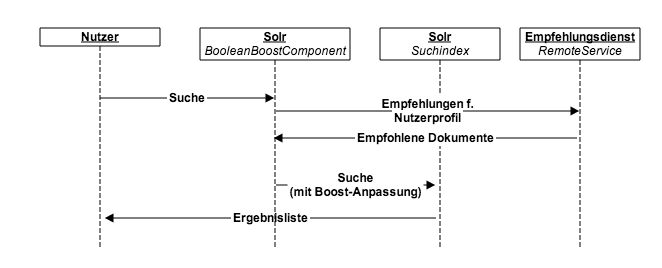
\includegraphics[width=\textwidth]{Abbildungen/search-rec1.png}
    \caption[Flussdiagram - externe Empfehlungen]{\footnotesize Flussdiagramm: Personalisierung von Suchanfragen über einen externen Empfehlungsdienst.}
    \label{fig:seq-extern-recommender}
\end{figure}

Wie in \ref{fig:seq-extern-recommender} dargestellt, wird die ursprüngliche Suchanfrage des Nutzers innerhalb der Komponente zunächst unterbrochen, um für das entsprechende Nutzerprofil die Empfehlungen vom externen Dienst berechnen zu lassen. Enthält die Antwort des Dienstes eine Liste von Empfehlungen, so wird diese innerhalb der Komponente in eine Solr-Anfrage, in diesem Fall einen \textit{BooleanQuery}, umgewandelt. Innerhalb des \textit{BooleanQuery} wird über \textit{TermQuery}-Elemente jeweils die Empfehlung für ein einzelnes Dokument der entsprechenden Solr-DokumentenID zugeordnet. Die so generierte Liste wird mit der ursprünglichen Anfrage verknüpft und entsprechend weiterverarbeitet. Die Kombination beider Anfragen hat dann zur Folge, dass Dokumente aus den Empfehlungen über die Faktoren des \textit{TermQuery} entsprechend ``besser'' bewertet werden wenn sie in der Ergebnisliste der ursprünglichen Suchanfrage enthalten sind. Sind die empfohlenen Dokumente nicht Teil der Ergebnisliste, kann keine Personalisierung vorgenommen werden und die Gewichtung bzw. Sortierung der Ergebnisse erfolgt rein TF-IDF-basiert.

Zur Konfiguration der Komponente stehen folgende Parameter zur Verfügung:
\begin{itemize}
\item \textit{boostBase} - Normalisierungswert bei der Dokumentenboost-Berechnung. ( $\alpha$ aus Formel (\ref{form:myscore0}) ).
\item \textit{boostAmount} - Menge der zu bildenden Empfehlungen
\item \textit{boostInline} - Schaltet die Integration in die ursprüngliche Anfrage ab und zeigt nur die Empfehlungen.
\end{itemize}

Die Verarbeitung kann hierbei komplett in der Vorverarbeitungsphase von Apache Solr erfolgen, so dass die eigentlichen Suchanfragen auch von innerhalb von Solr in Zwischenspeichern gehalten werden können und wiederholte Anfragen erbeblich schneller verarbeitet werden können.

\subsubsection{Integrierte Empfehlungsdienste} \label{sec:implmodelcalc}

Die Implementierung von Empfehlungen mit Hilfe von Element-Featurevekoren, wurde innerhalb der \textit{SimilarityBoost}-Komponente implementiert.  Die Verarbeitung einer Suchanfrage wird in Abbildung  \ref{fig:seq-intern-recommender} dargestellt.

\begin{figure}[H]
  \centering
    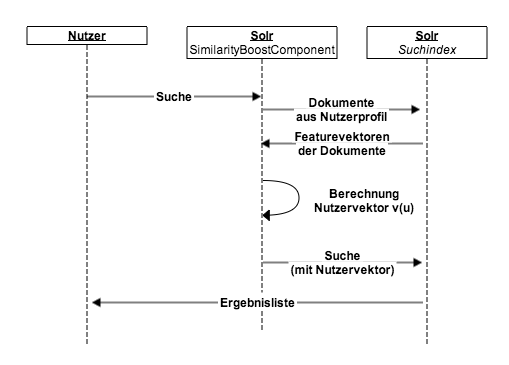
\includegraphics[width=0.77\textwidth]{Abbildungen/search-rec2.png}
    \caption[Flussdiagram - interne Empfehlungsbildung]{\footnotesize Flussdiagramm: Personalisierung von Suchanfragen über Featurevektoren im Suchindex.}
    \label{fig:seq-intern-recommender}
\end{figure}

Nachdem die Komponente die Anfrage des Nutzers erhalten hat, muss zunächst über eine zusätzliche Anfrage, die Liste der Dokumente des Nutzerprofils aus dem Suchindex gelesen werden. Mit Hilfe dieser Liste kann dann, der Nutzervektor $v(u)$ wie in Formel \ref{form:anonuser} gebildet werden. Danach kann die ursprüngliche Anfrage weiterverarbeitet werden.

Da die Konfiguration der Komponente (vgl. Listing \ref{lst:similardocs}) die weitere Verarbeitung von $v(u)$ (im Listing als \textit{\$features} bezeichnet) bestimmt, kann die Personalisierung bzw. Empfehlungsbildung unabhängig von der \textit{SimilarityField}-Komponente erfolgen. Das in Listing \ref{lst:similardocs} gezeigte Beispiel nutzt die Distanz zwischen den Dokumentenvektoren $w(i)$ und dem Nutzervektor $v(u)$ um für den Nutzer relevante Dokumente zu bevorzugen.

Da der größte Teil der Empfehlungsbildung innerhalb der normalen Apache Solr Komponenten erfolgt, beschränkt sich die Konfiguration der \textit{SimilarityField}-Komponente auf die Benennung des Featurevektoren-Feldes über den \textit{similarityField} Parameter. Alle weiteren Verarbeitungsschritte und Parameter werden innerhalb der \textit{solrconfig.xml} direkt angegeben.

\subsection{Systemaufbau}

Für die in Abbildung \ref{fig:system_rough} skizzierten Systembestandteile wird im Folgenden die gewählte Technologie erläutert und mit möglichen Alternativen verglichen. 

\subsubsection{Tracker} \label{sec:tracker-impl} Die Aufzeichnung der Interaktionen von Nutzer und Webseite, wurde mit Hilfe eines eigenen Java Servlets umgesetzt. Die Funktionalität des Trackers beschränkt sich auf das Erfassen von Interaktionen eines Nutzers innerhalb einer JavaScript-Bibliothek und die Weitergabe dieser innerhalb des Servlets. Da die Daten dem Anwendungsfall entsprechend gespeichert werden können, ist der Aufwand bei der weiteren Verarbeitung sehr gering. 

Da ein ``Datensatz'' einer Komponente der in Tabelle \ref{tab:user-item-ratings} gezeigten Matrix entspricht, enthält dieser auch ähnliche Daten. Für den Nutzer wird jeweils eine ID für die aktuelle Session, eine sessionübergreifende ID und (falls bekannt) den Account im System aufgezeichnet. Für das Element bzw. Produkt wird die SKU-ID aufgezeichnet und ggf. eine Produktgruppen-ID. Die Information über die Art der Interaktion wird in textheller Form gespeichert. In der Summe besteht ein einzelner Datensatz so aus ca. 114-150 Byte. Die Weitergabe dieser Daten erfolg über die im Abschnitt \ref{sec:datatransp} beschriebene Transporttechniken. Der Quellcode der Komponente ist unter \todo{Reg zum Tracker-Repo} verfügbar. 

Wichtigste Alternative zur Implementierung eines eigenen Dienstes wäre die Nutzung bzw. Auswertung schon vorhandener Daten aus Serverlogs und von externen Trackingdiensten (zB. Google Analytics) gewesen. Da dies allerdings mit sehr hohen Aufwand bei der Datenaufbereitung verbunden wäre und da nicht in jedem Anwendungsfall auf entsprechende Logs zurückgegriffen werden kann, wurde auf diese Art der Datengewinnung zunächst verzichtet.

\subsubsection{Datenhaltung} Für die dauerhafte Speicherung der aufgezeichneten Daten wurde zunächst auf die Verwendung eines verteilten Dateisystems (vgl. Abschnitt \ref{sec:hfs}) verzichtet. Da der Betrieb eines entsprechenden Serverclusters hohe Wartungskosten erzeugt hätte, wurde die lokale Speicherung der Daten und die bedarfsgemäße Nutzung von Amazon Web Services gewählt. Dies ermöglicht die MapReduce-basierte Verarbeitung der Daten (vgl. Abschnitt \ref{sec:mapred}) ohne dedizierte Hardware vorhalten zu müssen.

Der Kostenunterschied kann mit Hilfe der folgenden Rechnung veranschaulicht werden. Geht man von 50GB an aufgezeichneten Nutzdaten pro Jahr aus, erzeugt die Speicherung dieser Datenmenge zur Verarbeitung innerhalb des \textit{Amazon Simple Storage Services} (S3) Kosten von ca. \EUR{6} pro Transfer (Upload+Download). Würde man zur weiteren Verarbeitung drei \textit{Amazon Elastik Compute Cloud} \textit{m2.xlarge} Instanzen für einen Tag nutzen, entstünden Kosten von ca. \EUR{100} pro Tag \footnote{Als Vergleichswert wurde die unter http://calculator.s3.amazonaws.com/calc5.html am 01.08.2013 gezeigten Tagespreise genutzt}. Die Kosten von wöchentlichen Neuberechnungen innerhalb dieser Infrastruktur entsprechen damit ca. der Hälfte der anfallenden Kosten zur Anmietung ähnlicher Ressourcen bei normalen Hosting-Anbietern.

\subsubsection{Datentransport} \label{sec:datatransp} Zum sicheren Transport der Daten zwischen Tracker und der Datenhaltung wird \textit{Apache Flume} genutzt. Es implementiert ein einfaches \textit{Message Queue} System welches sicherstellt, dass alle Daten einer Quelle (Tracker) auch auf allen Senken (Datenhaltung) geschrieben wurden bevor diese das System verlassen. Im Vergleich zur direkten Speicherung der Daten auf einer entsprechenden Festplatte, bietet Apache Flume die Möglichkeit mit mehrere Quellen oder mehrere Senken zu arbeiten und Datenströme zu verteilen bzw. zusammenzufassen. Neben dem lokalen Dateisystem unterstützt Apache Flume zudem auch HDFS-Senken und Amazon S3-Senken. Dank dieser Eigenschaften wird sowohl die horizontale Skalierung des Trackers auf mehrere Knoten vereinfacht, als auch die Anbindung anderer, dem Anwendungsfall entsprechender, Datenhaltungssysteme.

Alternative Message Queue Systeme wie etwas Rabbit MQ oder Active MQ wurden nicht betrachtet. 

\subsubsection{Datenaufbereitung} Die Vorverarbeitung der Daten wurde mit \textit{Apache Pig} umgesetzt. Es stellt eine dem Anwendungsfall angepasste Datenflusssprache, das sog. \textit{Pig Latin}, zur Verfügung (Beispiel siehe Listing \ref{lst:pigprofiles}). Die darin beschriebenen Operationen werden zur Verarbeitung in \textit{Apache Hadoop} kompatible \textit{MapReduce} Operationen kompiliert und sind so ohne weitere Anpassungen verteilt ausführbar.  Damit ermöglichht es, die Anwendung der in Abschnitt \ref{sec:mapred} beschriebenen Methoden um Skalierbarkeit zu gewährleisten. Die in \textit{Pig Latin} beschriebenen Datenverarbeitungsprogramme lassen sich über \textit{Amazon Elastic MapReduce} auch für Daten nutzen welche in \textit{Amazon S3} gehalten werden. \citep{Lin2012}

 \lstinputlisting[caption=Apache Pig Beispielscript zur Kombination von Nutzerprofiledaten,float,language=bash,label={lst:pigprofiles}]{Listings/pig-profiles.txt}

Eine umfassende Dokumentation der Möglichkeiten von \textit{Apache Pig} zur Datenverarbeitung bietet \citep{gates2011programming}. Die Integration von Aufgaben des maschinellen Lernens mit  \textit{Apache Pig} wird in  \citep{Lin2012} beschrieben.

Alternative \textit{MapReduce} Implementierungen in Java oder \textit{Apache Hive} wurden nicht betrachtet.

\subsubsection{Empfehlungsdienst} Wie im vorangegangen Abschnitt \ref{sec:mahout} beschrieben, wurde die Integration der Empfehlungs- und Modellberechnung mit \textit{Apache Mahout} vorgenommen. 

Die Vorberechnung der Ähnlichkeitsmodelle (vgl. Abschnitt \ref{sec:scalefiltering}) wird als verteilte Berechnung wie in Listing \ref{lst:useritemmodelprep} ausgeführt. Um die darin berechneten Modelle direkt im Empfehlungsdienst nutzen zu können, wird die Ähnlichkeitsmatrix in einem Nachverarbeitungsschritt (vgl. \textit{PairSimilarityJob}) in ein textuelles Austauschformat überführt. Dieses Austauschformat wird dann über das in Mahout vorhandene \textit{FileDataModel} in den Empfehlungsdienst geladen. Dieser wird als Webservice über eine HTTP-Schnittstelle (vgl. \textit{com.aoe.cf.recommender.RemoteService}) zur Verfügung gestellt. Die Matrixfaktorisierung wird wie in Listing \ref{lst:factorgenerator} gezeigt, mit den in Abschnitt \label{sec:myrecommend} beschriebenen Methoden durchgeführt.

Die Evaluation der Ergebnisse beider Vorberechnungsmethoden erfolgt über die ergänzend bereitgestellten Evaluationsprogramme. In beiden Fälle werden die Empfehlungsergebnisse für zuvor gespeicherten Testdaten (vgl. Listing \ref{lst:dataprep}) mit den tatsächlich bekannten Daten vergleichen um die in Abschnitt \ref{sec:measures} beschriebenen Metriken zu generieren.

\subsubsection{Suche}

Die Integration mit der Suche erfolgt wie in Abschnitt \ref{sec:searchrelevance} beschrieben. Die Empfehlungsdienste auf Basis des Webservices werden wie in Listing \ref{lst:solrconfig} über die \textit{booleanBoost}-Komponente eingebunden und konfiguriert. Zur Integration der featurebasierten Empfehlungen wird die \textit{similarityField} Komponente eingebunden und über die erweiterte Boost-Konfiguration wie in Listing \ref{lst:similardocs}  zur Personalisierung benutzt.

Zur Erfüllung der in Abschnitt \ref{sec:userstories} beschriebenen Anwendungsfälle können beide Komponenten auch so integriert bzw. konfiguriert werden, dass Empfehlungen direkt ``ausgegeben'' werden oder dass Empfehlungen nicht für reale Nutzerprofile und stattdessen für anonyme Produktlisten generiert werden. Da beide Komponenten direkt in den Verarbeitungsablauf von \textit{Apache Solr} integriert sind, obliegt die Ausgestaltung der konkreten Anwendungsfälle der konkreten Applikation und wird zur Wahrung des Umfangs nicht näher betrachtet.

%\subsubsection{Datenhaltung}
%\subsection{Systemaufbau}
%\subsubsection{Tracking-Pixel}
%\subsubsection{Datenhaltung}
% Siehe "Programming Pig" S 19.2
%\sub

\newpage \section{Evaluation}\label{sec:evaluation}

% \textit{Wie wird gemessen, welche Ergebnisse waren zu erwarten, was wurde erreicht. Warum gibt es Abweichungen, welche Probleme enthält die Messmethode.\todo{raus}}

Im folgenden Abschnitt wird die implementierte Lösung hinsichtlich der Leistungs- und Qualitätsanforderungen (vgl. Abschnitt \ref{sec:requirements}) evaluiert. Ergänzend zur Bestimmung und Beschreibung der Ergebnisse werden mögliche Probleme der Evaluation und des Systemaufbaus in Abschnitt \ref{sec:discuss} beschrieben.

Da zum Zeitpunkt der Fertigstellung der Arbeit noch kein ausreichend umfangreicher realer Datensatz zur Verfügung stand, wurde der frei verfügbare MovieLens 1M \citep{movielens1m} Datensatz genutzt. Dieser besteht aus ca. 1 Million Nutzerbewertungen von 3.900 Nutzern für 6040 Kinofilme. Für jeden Nutzer liegen zudem mindestens 20 Bewertungen vor. Der Datensatz wurde gewählt, da er bereits in zahlreichen Publikationen zur Ergebnisevaluation genutzt wird  (u.a.  \citep{Cacheda2011}, \citep{Candillier:2008}, \citep{Paterek07} und \citep{Herlocker:1999:AFP:312624.312682}) und so gute Vergleichbarkeit bei den Ergebnissen gegeben ist.

Um zudem realistische Leistungsmessungen der Suchlösung durchführen zu können, war es notwendig neben den reinen Bewertungsdaten textuelle Inhalte im zu untersuchenden Solr-Index zu speichern. Zu diesem Zweck wurde der Index auf Basis der korrespondierenden Filmdaten aus offenen Datenquellen\footnote{http://www.themoviedb.org/, http://mymovieapi.com/} gefüllt, so dass pro Film zwanzig verschiedene Textfelder u.a. mit Titel, Beschreibungen, Schauspielernamen und Stichworten zum Film gefüllt waren. Die Apache Solr Konfigurationsdateien\footnote{Git Repository Solr Konfiguration: https://git.gitorious.org/recommend/solr-config} (vgl. Abschnitt \ref{sec:solr}) sind, ebenso wie die Skripte zur Indexing der textuellen Informationen\footnote{Git Repository Indexierung: https://gitorious.org/recommend/imdb-index} und der zugehörigen Featurevektoren, zur besseren Nachvollziehbarkeit in einem Respository.

\newpage
\subsection{Ergebnisse}

\subsubsection{Leistung}\label{sec:performance}

Zur Bestimmung der Leistung wurden jeweils die in Abschnitt \ref{sec:requirements} beschriebenen Anforderungen an die Anfragen pro Sekunde für die einzelnen Dienste geprüft. Als Referenzsystem wurden mit dem Betriebssystem Ubuntu Server 12.04 betriebener Server genutzt.  Die Hardware der Servers wurde mit 16 GB RAM und einem Dual-Core Intel Xeon E31275 so gewählt, dass diese mit Amazon EC2 m1.xlarge Instanzen\footnote{Amazon EC2 Instanz-Typen: http://aws.amazon.com/de/ec2/instance-types - geprüft am 13.09.2013} vergleichbar sind. Als Webserver bzw. Servlet-Container wurde Jetty\footnote{siehe: http://www.eclipse.org/jetty/} Version 8 hinter einem Nginx \gls{Reverse Proxy} genutzt.

Die Testpläne wurden mit Apache Jmeter\footnote{siehe: http://jmeter.apache.org/} aufgebaut und durchgeführt. Sie werden in einem eigenen Repository zur besseren Nachvollziehbarkeit zur Verfügung gestellt\footnote{Git Repository: Performance Tests: https://gitorious.org/recommend/performance-tests}. Um eine möglichst gleichförmige Ausführung zu gewährleisten wurden die Tests automatisch durchgeführt (vgl. Listing \ref{lst:jmeterscript}). Die einzelnen Messungen liefen, wenn nicht anders angegeben, jeweils 60 Sekunden mit einer vorgelagerten 30-sekündigen Ruhephase. Alle Systeme wurden im gleichen Rechenzentrum genutzt, um den Einfluss von Netzwerklatenzen zu vermindern.

Die vollständige Auflistung der Messergebnisse für die einzelnen Systembestandteile und Konfigurationen befindet sich in Anhang \ref{app:performance}.

 \lstinputlisting[caption=Script zur systematischen Ausführung von Leistungstests mit Apache Jmeter,language=bash,label={lst:jmeterscript}]{Listings/jmeter.txt}

\newpage

\paragraph{Tracker} Da die große Anzahl der zu erwartenden Anfragen auch eine sehr großen Zahl gleichzeitiger Verbindungen erfordert, wurden neben dem möglichen Durchsatz auch die maximal möglichen parallelen Verbindungen ermittelt. Um der normalen Nutzung des Dienstes zu entsprechen, wurden zufällige Trackingevents über die HTTP-Schnittstelle an den Dienst gesendet und die entsprechende Antwort geprüft.

Die Erwartung, dass der Dienst ab einer bestimmten Anzahl paralleler Anfragen neue Verbindungen nicht mehr annehmen kann und diese abweisen muss, wurde erfüllt. Wie in Abbildung \ref{fig:chart_tracker} deutlich wird, ist diese Schwelle bei ca. 350 gleichzeitigen Verbindungen erreicht. Dies hat zur Folge, dass der maximale Durchsatz stark einbricht. Ab ca. 600 parallelen Anfragen kommt es zu Verbindungsabbrüchen, was durch die ebenfalls abgebildeten Fehlerquote gezeigt wird.

Die Anforderungen an den maximalen Durchsatz erreicht bzw. übertrifft der so betriebene Dienst. Zum Test von dauerhafter Stabilität wurden, ergänzend zu den Test der Lastspitzen, auch zwei dreißigminütige Tests mit  50 bzw. 100 Anfragen pro Sekunde durchgeführt. In beiden Tests konnten keine Fehler oder Verbindungsabbrüche gemessen werden.

\begin{figure}[htb]
  \centering
    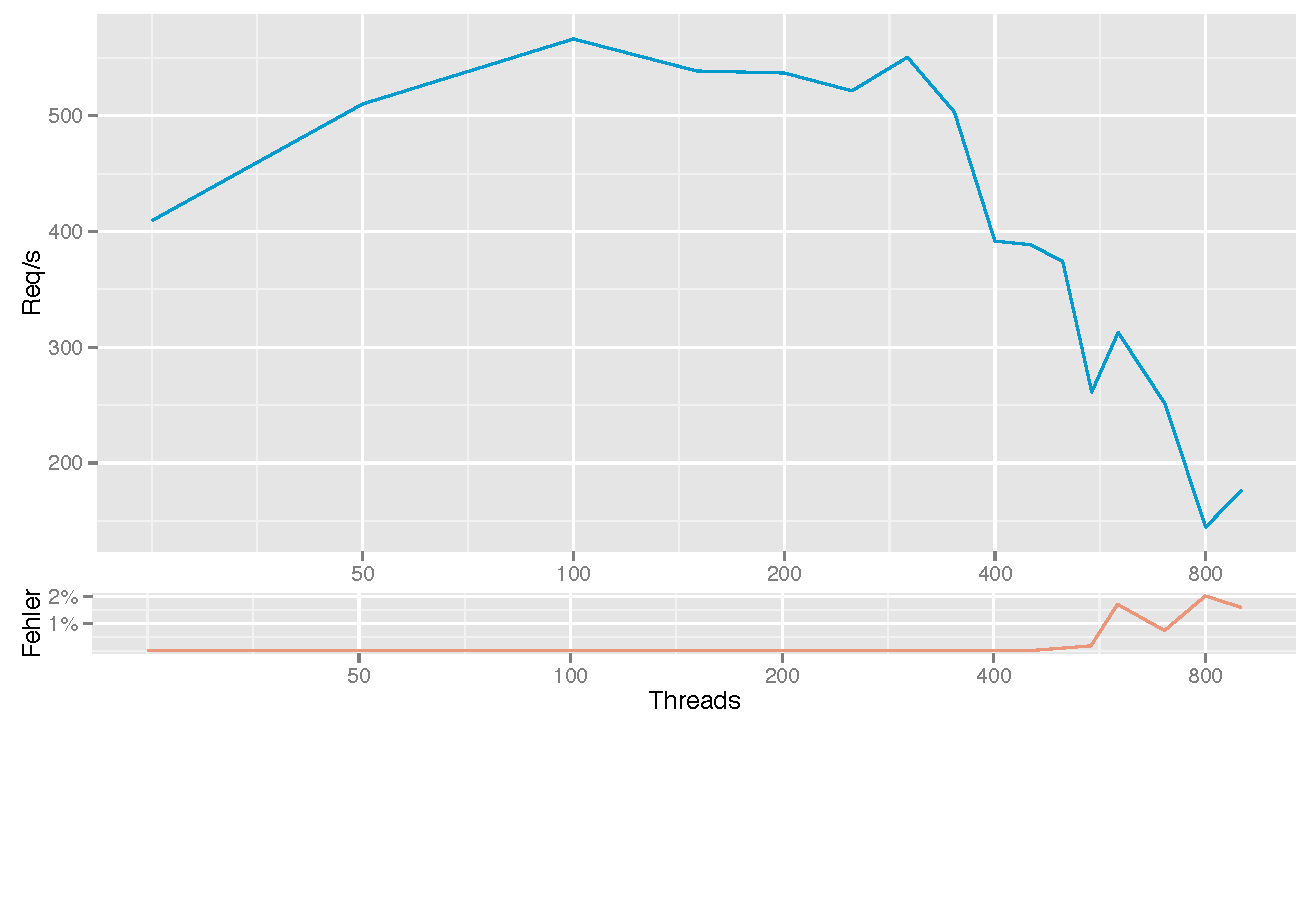
\includegraphics[width=0.9\textwidth]{Abbildungen/tracker.pdf}
    \caption[Leistung Tracker]{Trackerleistungsdiagramm - Gegenüberstellung der Anzahl der parallel genutzten Threads, der erzielten Leistung und der Fehlerquote. { \scriptsize (eigene Darstellung)}}
    \label{fig:chart_tracker}
\end{figure}

\paragraph{Apache Solr} Zur Messung der Leistungsfähigkeit der verschiedenen Personalisierungsmethoden wurden die Leistungswerte der Suche ohne Personaliserung mit denen der beiden Personalisierungsmethoden gegenübergestellt. Da bei großen Daten- bzw. Anfrageaufkommen die Suchanfragen wie in Abschnitt  \ref{sec:solrshards} beschrieben auch auf mehrere Backend-Server verteilt werden können, wurde die Evaluation mit bis zu drei Solr-Instanzen durchgeführt. Um eine maximale Lesegeschwindigkeit zu ermöglichen, waren die Instanzen ohne Sharding, d.h. mit voller Daten-Replikation, konfiguriert. Bei der Personalisierung mittels Webservice wurde zudem für jede Solr-Instanz ein eigener Recommendation-Service aufgesetzt. Da der Suchindex durch den geringen Umfang der Beispieldaten von Solr vollständig im Speicher gehalten werden kann, waren Durchsatzgrößen von 200 Requests pro Sekunde pro Solr-Instanz zu erwarten. Vergleichbare Ergebnisse werden in \citep{Rappold2013} bei der Nutzung einer RAM-Disk beschrieben.

Die Anfragen wurden auf Basis von zufällig gebildeten Suchausdrücken von bis zu 5 Wörtern gestellt. Die dafür verwendeten Wörter wurden so gewählt, dass deren Dokumentenfrequenz (vgl. Abschnitt \ref{tfidf}) mindestens 10 und maximal 20 betrug. Dadurch sollte sichergestellt werden, dass alle Ergebnislisten ähnlich umfangreich und nicht leer waren. Ebenso wurden die für die Personalisierung notwendigen Nutzerprofile zufällig aus zwei bis zehn Elementen gebildet. Die Vermeidung von leeren Ergebnislisten und Profilen mit nicht vorhandenen Elementen sollte dabei vor allem der besseren Vergleichbarkeit dienen.  Um mögliche Probleme sichtbar zu machen, wurden leere Ergebnislisten ebenso wie Verbindungsabbrüche als Fehler aufgezeichnet.

Abbildung \ref{fig:chart_solr} stellt die Ergebnisse der Leistungsmessung gegenüber. Wie bei der Messung der Tracker-Leistung wurden ebenfalls verschiedene Parallelitätsgrade und die damit erzielbare Leistung für die verschiedenen Konfigurationen gemessen. Die in Abschnitt \ref{sec:requirements} beschriebenen Anforderung ist als graue Linie im Diagramm kenntlich gemacht. Da diese im Vergleich zum Tracker geringer ist und damit auch die zu erwartende Anzahl paralleler Anfragen erheblich niedriger sein wird, wurden die gewählten Parallelisierungsstufen anders verteilt. Um die Auswirkungen großer Verbindungszahlen dennoch zu zeigen, wurde ebenfalls bis in den Bereich von 900 parallelen Threads gemessen.

\begin{figure}[htb]
  \centering
    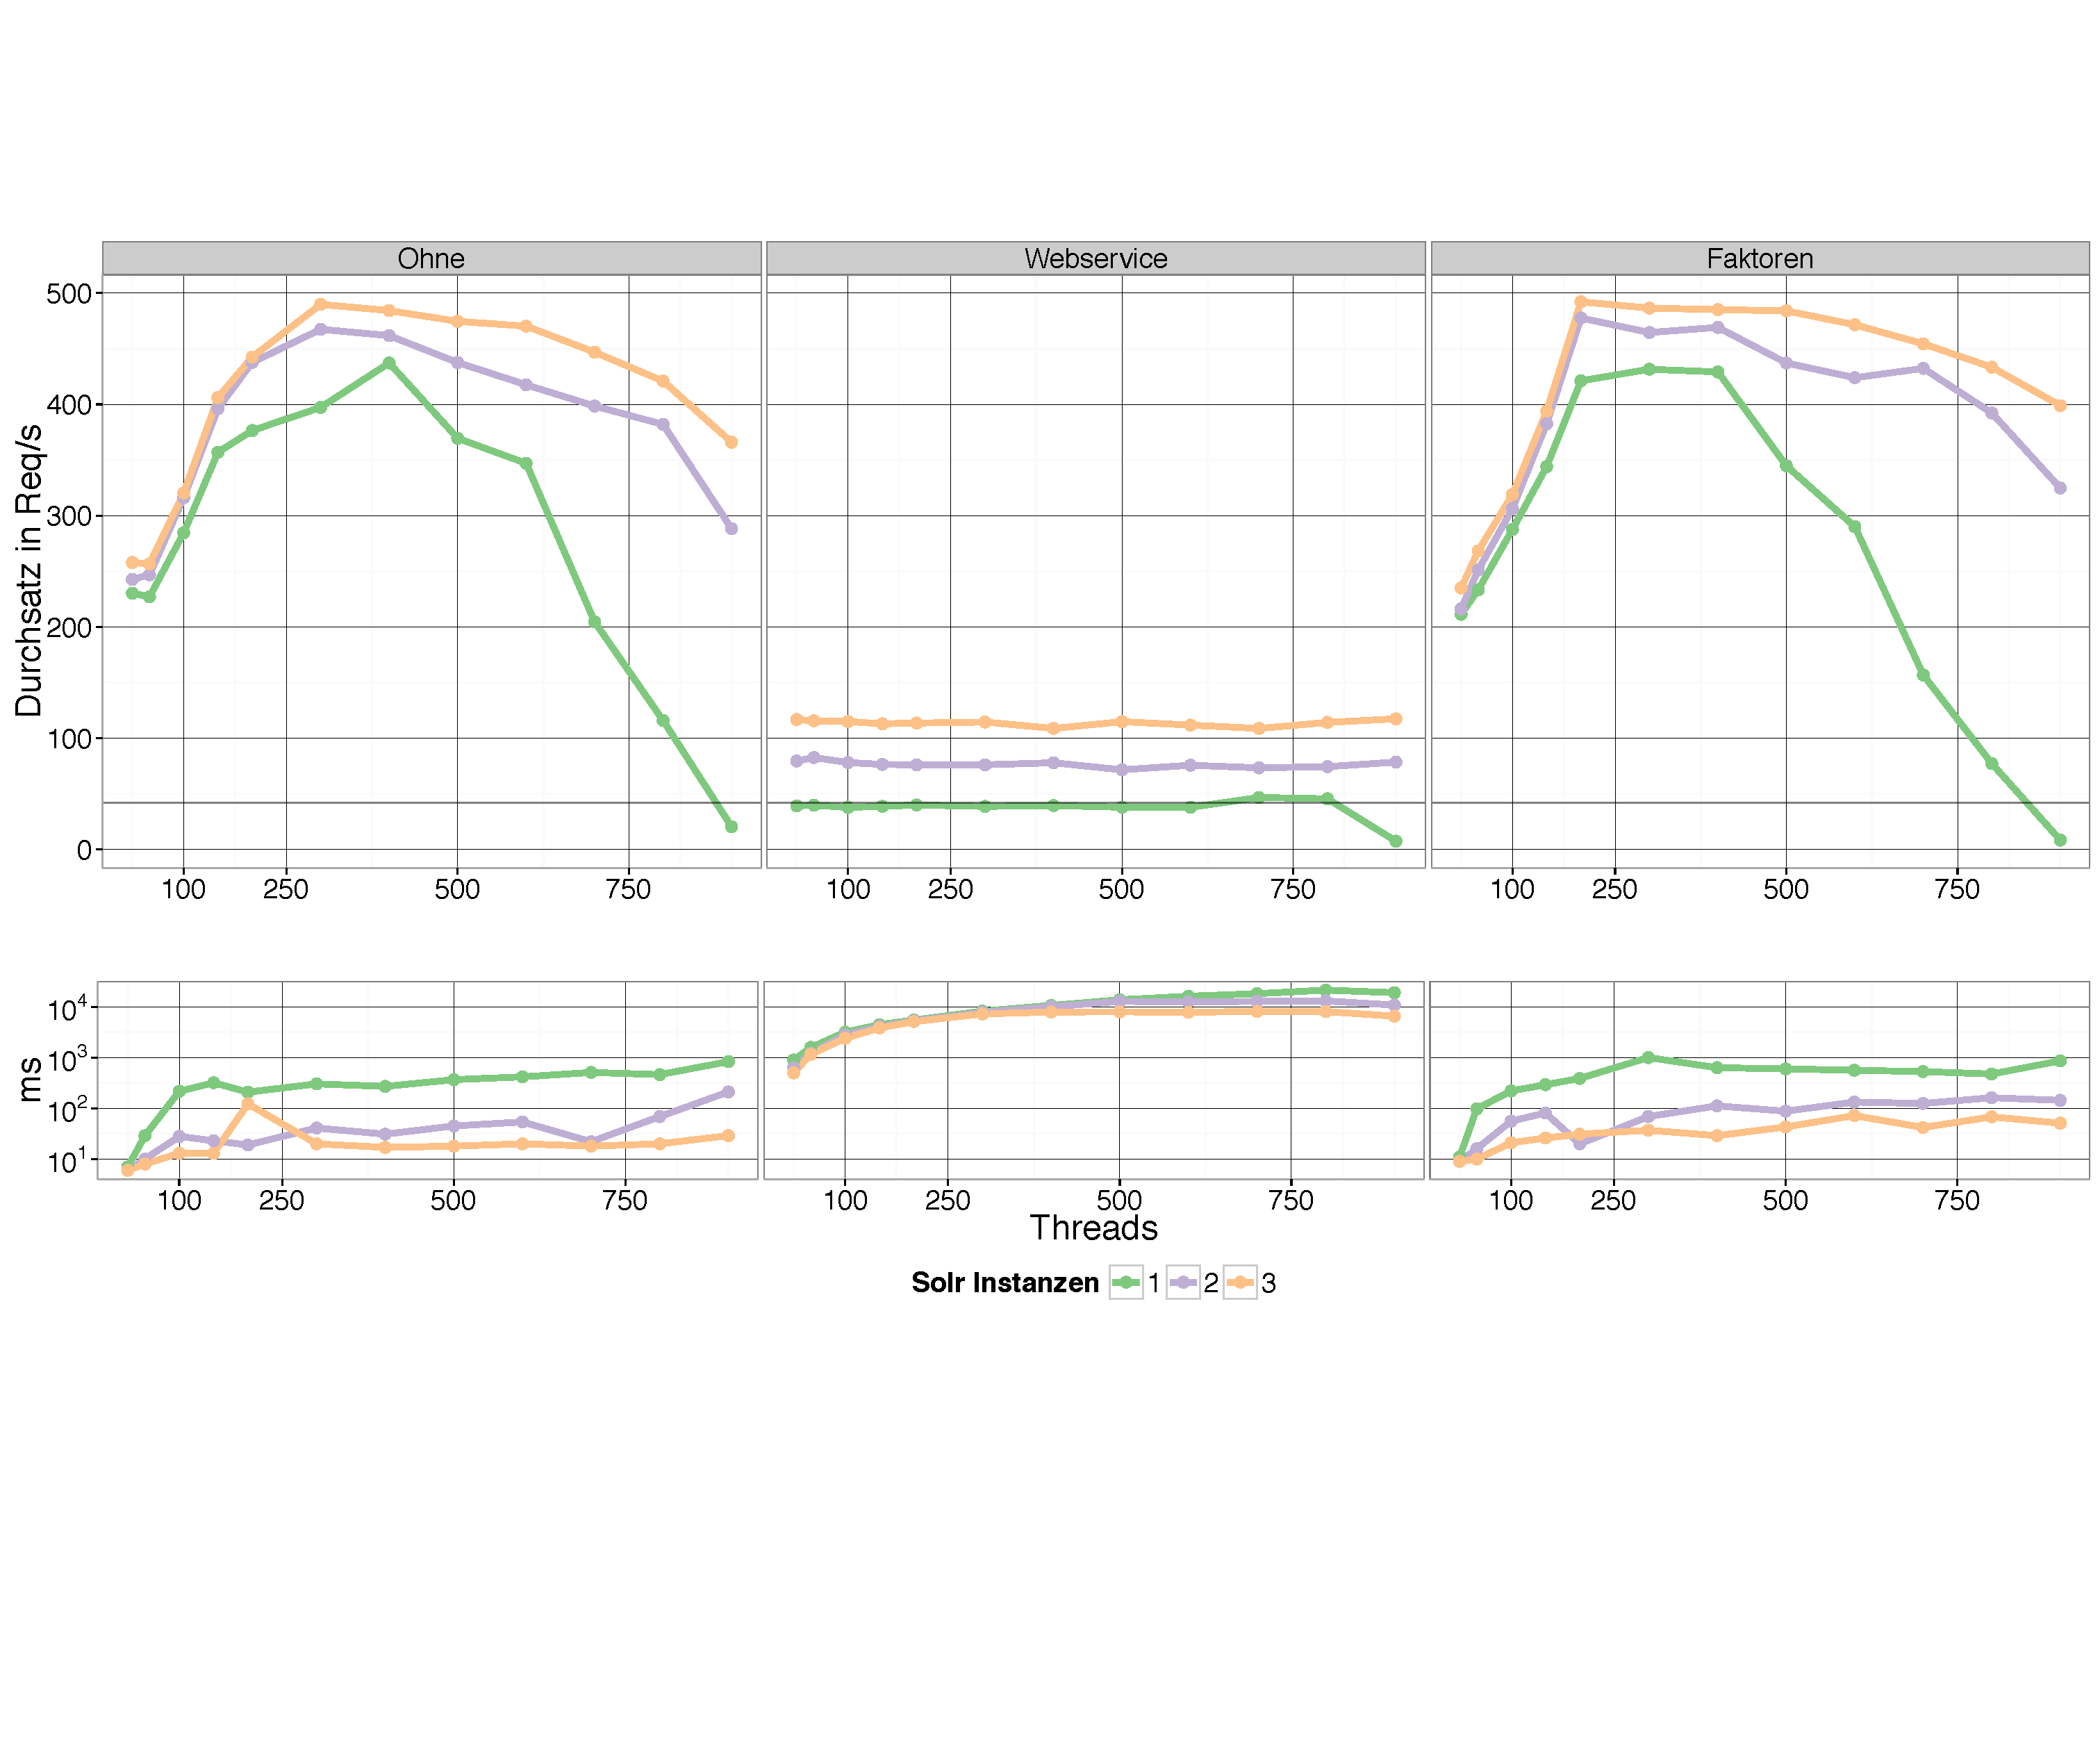
\includegraphics[width=\textwidth]{Abbildungen/personalisierung.pdf}
    \caption[Leistung d. personalisierten Suche]{Leistungsvergleich der Solr-Instanzen mit verschiedenen Personalisierungslösungen für verschiedene Parallelisierungs- und Skalierungsstufen.  {\scriptsize (eigene Darstellung)} \\ { \footnotesize \textbf{Oben}: Leistungsdaten in Requests / Sekunde -- \textbf{Unten}: 90\%-Dezil der Antwortzeiten in Millisekunden.}} 
    \label{fig:chart_solr}
\end{figure}

Entgegen der Erwartung, dass die Leistung des unpersonalisierten Apache Solr mit jeder Instanz nahezu linear skaliert, zeigt sich die Auswirkung weiterer Instanzen erst bei der Steigerung der parallelen Anfragen.  Die geringe Leistung des nicht auf Parallelität optimierten Webservices spiegelt sich erwartungsgemäß in den erheblich niedrigeren Leistungswerten der entsprechenden Personalisierungslösung. Wie sich zudem zeigt, skaliert die Lösung mit weiteren Instanzen linear. Die auf Faktoren basierte Personalisierung zeigt den Erwartungen entsprechend das gleiche Skaliersungsverhalten wie die Solr-Instanzen ohne Personalisierung. Da allerdings für einige Dokumente kein Featurevektor gelernt werden konnte, zeigen die Ergebnisse eine nahezu konstante Fehlerquote von 0.3\% im Zusammenhang mit den entsprechenden Dokumenten.

Das ebenfalls in Abbildung \ref{fig:chart_solr} dargestellte 90\%-Dezil der Antwortzeiten bestätigt den deutlichen Leistungsunterschied bei der Verwendung des ausgelagerten Dienstes. 
In den gemessenen Latenzwerten zeigt sich zudem das erwartete Skalierungsverhalten bei allen Lösungen und für alle Parallelisierungsgrade.

Der zu erwartende Einbruch des Durchsatzes bei einer großen Zahl von parallelen Verbindungen zeigt sich, wie bei der Leistungsmessung des Trackers, ebenfalls. Der Schwellwert liegt zwischen 400 und 500  Verbindungen. Durch Verbindungsabbrüche hervorgerufene Fehler treten ab einer Anzahl von 600 parallelen Verbindungen auf. Die in Abschnitt \ref{sec:requirements} beschriebenen Anforderungen werden von allen drei Personalisierungslösungen erreicht.

\subsubsection{Empfehlungsqualität}

Zur Messung der Qualität wurden die in Abschnitt \ref{sec:qa_rmse} beschrieben Maße zur mittleren (\acs{MAE}) und zur quadratischen (\acs{RMSE}) Abweichung genutzt. Bestimmt wurden diese für elementbasierte Nachbarschaftmodelle mit verschiedenen Distanzmetriken und für den im Rahmen der Arbeit implementierten NSVD2 Algorithmus. Als weitere Referenzwerte wurde zudem die Qualität des in Apache Mahout vorhandenen SVD-Recommenders und die eines Zufalls-Recommendes gemessen.

Das Training der evaluierten Modelle wurde mit 90\% des Datenbestandes durchgeführt. Die restlichen 10\% der Daten wurden für die Evaluation genutzt. Da es innerhalb des MovieLens 1M Datensatzes keine feste Aufteilung in Trainings- und Kontrolldaten gibt, wurde die Aufteilung zufällig vorgenommen. Um zu verhindern, dass die Aufteilung der Daten die Ergebnisse beeinflusst, wurden die Mittelwerte von 10 Berechnungen mit verschiedenen Aufteilungen für jede Methode gebildet. Die dabei gemessenen Werte sind in Tabelle \ref{tab:rmse-eval} aufgelistet.

\vfill
\begin{table}[h]
  \centering
  \begin{minipage}[b]{5in}
  \begin{tabular}{ | l | l || r | r | }
  %\cline{2}
  \hline
  \textbf { Alogrithmus } &   \textbf { Distanzmaß } &   \textbf { RMSE } &   \textbf { MAE } \\ \hline
  \multirow{4}{*}{Elementbasierte Modelle}  & Kosinus Ähnl. & 0.9730 & 0.7705 \\ 
 & Euklid. Distanz & 1.1131 & 0.8945\\   
 & Jaccard-Koeff. & 0.9616 & 0.7611 \\
 & Pearson-Korr.  & 0.9723 & 0.7553 \\ \hline
  NSVD2 & - & 	0.9840  & 0.8223 \\
  SVD &  - &	0.9062 & 0.7383 \\ \hline
  Zufall & -	&	1.7358 & 1.3689 \\ \hline
  \end{tabular}
  \caption{\footnotesize Evaluationsergebnisse der vorgestellten Recommender-Algorithmen mit Apache Mahout  (vgl. Abschnitt \ref{sec:filtermethods}). { \scriptsize (eigene Darstellung)}}
  \label{tab:rmse-eval}
\end{minipage}
\end{table}

Die auf Matrixfaktorisierung basierenden SVD und NSVD2 Modelle wurden mit 10-dimensionalen Featurevektoren trainiert. Die Laufzeit des Trainings war auf 10 Iterationen pro Feature begrenzt.

Die erzielten Ergebnisse entsprechen denen anderer Publikationen. Wie in \citep{Herlocker:1999:AFP:312624.312682} und \citep{Candillier:2008} wird bei den elementbasierten Nachbarschaftmodellen der Jaccard-Koeffizient bezüglich des \acs{RMSE} bevorzugt und die Pearson-Korrelation bezüglich des \acs{MAE}. Zudem zeigt sich in beiden Fehlermaßen, dass der euklidische Abstand keine geeignete Metrik für die vorliegenden Daten ist.

%Da die Evaluation in \citep{Paterek07} und \todo{cite} des NSVD2 Algorithmus nur auf andere, nicht öffentliche Datensätze durchgeführt wurden, war der direkte Vergleich von Ergebnissen mit anderen Veröffentlichungen für die faktorenbasierten Methoden NSVD2 und SVD bezüglich der MovieLens 1M nicht möglich. Dennoch

Der Vergleich der faktorenbasierten Methoden NSVD2 und SVD entspricht ebenfalls den Erwartungen. Übereinstimmend mit den Ergebnissen aus \citep{Paterek07}, bezüglich eines anderen Datensatzens und \citep{Cacheda2011} bezüglich des MovieLens 1M Datensatzes war es zu erwarten, dass NSVD2 schlechtere Ergebnisse liefert. Dass SVD bezüglich beider Qualitätsmaße bessere Ergebnisse liefert als die elementbasierten Nachbarschaftsmodelle bestätigt die Erwartungen aus \citep{Cacheda2011} und \citep{Koren:2009:MFT:1608565.1608614}.

% entsprechen die erzielten Ergebnisse den Erwartungen, dass SVD bezüglich der beiden Qualitätsmaße ein besseres Ergebnis liefert als die elementbasierten Nachbarschaftsmodelle (vgl. ). 

Der Vergleich aller Ergebnisse mit denen des zufälligen Empfehlungsdienstes zeigt, dass in allen Fällen erheblich bessere Ergebnisse erzielt werden können. Da keine quelloffene Referenzimplementierungen des NSVD2 Algorithmus existiert, ist dieser Vergleich notwendig, um einen funktionierenden aber schlecht parametrisierten von einem nicht-funktionalem Empfehlungsdienst zu unterscheiden. Da das Ziel der Qualitätstests nicht die Optimierung der Parameter für die Beispieldaten war und sich mögliche Erkenntnisse nur begrenzt auf andere Quellen übertragen lassen, wurden keine ergänzenden Evaluationen anderer Parameterkombinationen oder mit ergänzenden Maßen (vgl. Abschnitt \ref{sec:measures}) durchgeführt. \newpage

\subsubsection{Disjunkte Kanidatenlisten} \label{sec:disjunction_check}

Zur Untersuchung der in Abschnitt \ref{sec:disjunctcanidates} beschriebenen Problematik der disjunkten Ergebnislisten wurde die Größe der Schnittmenge der Ergebnislisten von Suche und Empfehlungsdienst bei der Personalisierung mittels Webservice untersucht. Wie in den vorangegangenen Abschnitten wurden dabei zufällige Suchen mit bis zu zwanzig Wörtern mit ebenfalls zufällig gebildeten Nutzungsprofilen betrachete. Von allen Suchergebnislisten wurden die ersten fünfzig Elemente ausgewertet und geprüft wieviele der dafür empfohlenen Elementen enthalten waren. Da zu erwarten war, dass die Größe der Schnittmenge vom Umfang der Empfehlungsliste abhängig ist, wurden vier verschiedene Größenkonfigurationen geprüft. Da die Größe der Suchergebnisliste vorwiegend davon abhängig ist, wieviele Elemente ein Nutzer sich ansehen möchte und dadurch nicht beliebig zur Konfiguration angepasst werden kann, wurde ihr Umfang nicht variiert.

Die Ergebnisse der Untersuchung werden in Abbildung \ref{fig:chart_disjunction} gegenübergestellt. Durch die zufällig gebildeten Suchbegriffe und den zudem fehlenden Kontext zum Nutzerprofil war zu erwarten, dass die Schnittmengen sehr gering sind. Diese Erwartungen wurden ebenso bestätigt wie die Annahme, dass mit zunehmendem Umfang der Empfehlungen auch die Größe der Schnittmenge steigt.

\begin{figure}[htb]
  \centering
    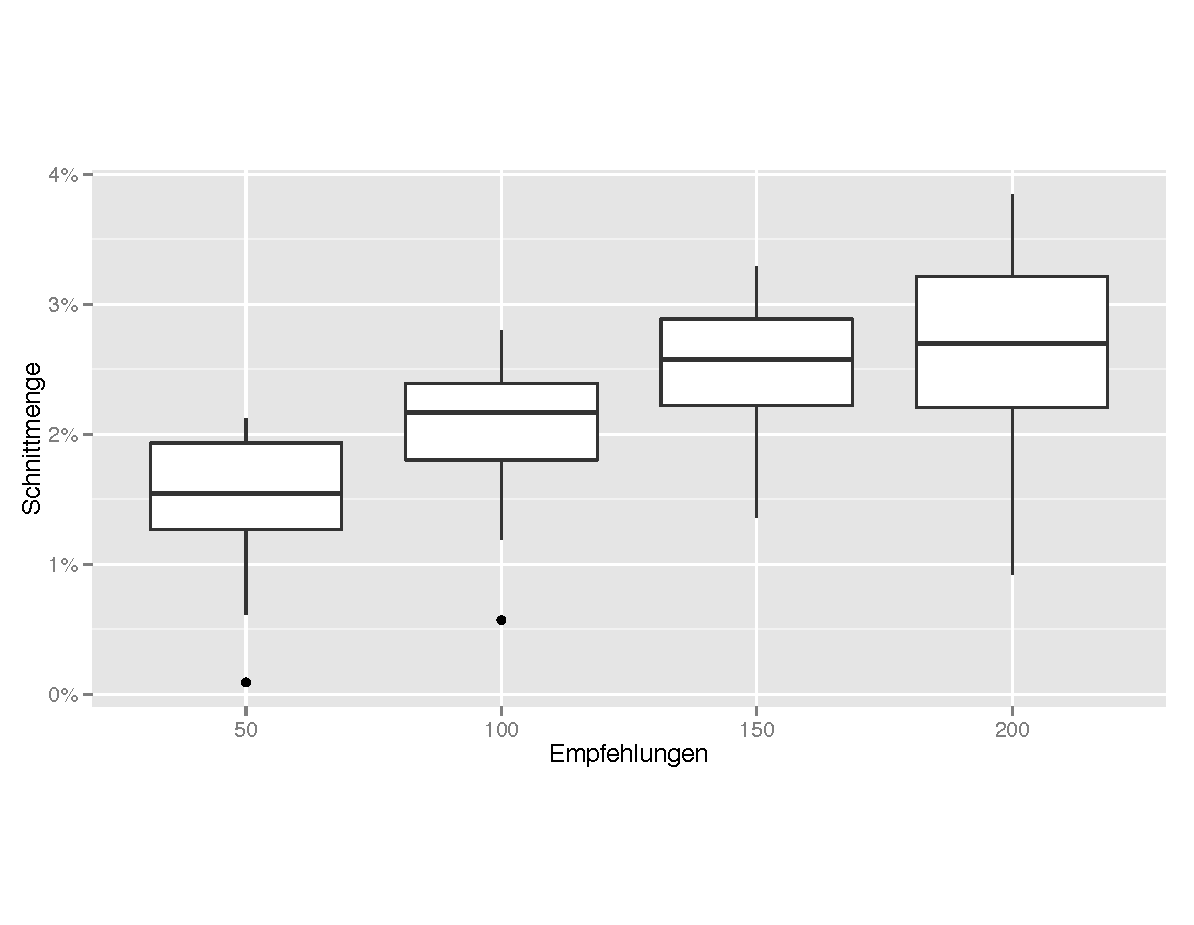
\includegraphics[width=0.75\textwidth]{Abbildungen/disjunction.pdf}
    \caption{Schnittmengenvergleich bei der Nutzung der Personalisierung mittels Webservice in Abhängigkeit der Empfehlungsgrößen {\scriptsize (eigene Darstellung)}}
    \label{fig:chart_disjunction}
\end{figure}

\subsection{Diskussion} \label{sec:discuss}

\paragraph{Skalierungsverhalten und Latenz} Da die Skalierbarkeit des Systems eines der wichtigsten Ziele der Arbeit darstellt, waren die umfassenden Tests aus Abschnitt \ref{sec:performance} notwendig und die erzielten Ergebnisse insgesamt mehr als zufriedenstellend. Die Zusammenstellung und Konfiguration der gewählten Systemkomponenten entspricht den in Abschnitt \ref{sec:requirements} beschriebenen Anforderungen. % Da alle Tests mit Standardkonfigurationen aller Bestandteile durchgeführt wurden, besteht neben den Möglichkeiten der horizontalen Skalierung ebenfalls Raum für weitere Optimierungen bezüglich der beschriebenen Plattform.

Das nicht erwartungsgemäße Skalierungsverhalten der Apache Solr-Instanzen bei geringen Parallelisierungsgraden weist auf ein mögliches Konfigurationsproblem der Testumgebung oder des Testwerkzeuges hin. Da die Tests ausschließlich von einem einzigen Quellsystem ausgeführt wurden, ist es zum Beispiel denkbar, dass diese nicht gleichmäßig verteilt wurden bis ein gewisser Schwellwert erreicht war. Ein weiterer Faktor, der in diesem Zusammenhang nicht näher untersucht werden konnte, ist die Dokumentengröße und mögliche Auswirkungen auf den erzielbaren Anfragen pro Sekunde. \citep{solrperformance} %\todo{Nicht soo besonders formuliert alles}

Die erzielte mittlere Latenz des Trackers und der Suchimplementierungen entsprachen den Erwartungen. Da normale Clientsysteme in der Regel nicht im gleichen Rechenzentrum angebunden sind, entspricht die Latenz nur begrenzt den realen Bedingungen. Zudem konnte sie davon profitieren, dass die Tests auf einem einzigen System durchgeführt wurden. Da eine größere Anzahl von Clientsystemen die Verwaltung der bestehenden Verbindung und Optimierungen auf der Ebene der Transportschicht erschwert, ist im praktischem Betrieb mit deutlich höheren Latenzwerten zu rechnen. Um diese Aspekte auch in die Tests einzubeziehen, sollten die Latenzwerttests ergänzend mit einer größeren Anzahl von Clientsystemen wiederholt werden. \citep{jetty2008}

\paragraph{Apache Solr} Die erwartungsgemäß guten Leistungs- und Latenzwerte der Apache Solr-Instanzen sind bei der beschriebenen Nutzung mit wenigen tausend Dokumenten nur bedingt übertragbar. Wird die horizontale Skalierung (vgl. Abschnitt \ref{sec:sharding}) mit einer Aufteilung der Daten in verschiedene Datenblöcke pro Backend-Knoten genutzt, lässt sich das im Rahmen der Evaluation bestätigte Verhalten nur eingeschränkt übertragen. Da der Umfang der im Suchindex gehaltenen Daten mit wenigen tausend Dokumenten die vollständige Replikation auf alle drei Solr-Instanzen erlaubt und da zudem davon auszugehen ist, dass der Index jederzeit vollständige im Dokumenten-Cache von Solr vorgehalten werden konnte, entsprachen die Leistungsdaten des nicht optimierten Testsystems denen eines optimierten Produktivsystems (vgl. \citep{Rappold2013}).  Durch den geringen Umfang des Indexes konnte zudem nicht geprüft werden, inwiefern die im Solr integrierten Caches weiterhin effizient arbeiten können. Es ist zum Beispiel naheliegend, dass zwischengespeicherte Suchergebnislisten, wegen unterschiedlicher Präferenzwerte, nicht zwischen verschiedenen Nutzern übertragen werden können und so die Effizienz der Zwischenspeicher wegen der Personaliserung nicht mehr gegeben ist (vgl. \citep{solrcache}). 

%\paragraph{Systembestandteile} 
%JVM Optimierung / J2EE Container / Plattform
\paragraph{Qualitätsmaße} Da die gute Vergleichbarkeit der Empfehlungsqualität im Vordergrund stand, wurden die in den Publikationen weiter verbreiteten Fehlermaße \acs{RMSE} und \acs{MAE} genutzt. Da in der praktischen Anwendung den Top-N Ergebnissen eine sehr hohe Bedeutung zugemessen wird, kann mit diesen Maßen kein direkter Schluss auf die Qualität eines Algorithmus in diesem Bezug getroffen werden. Aus diesem Grund ist es sinnvoll jeden Algorithmus auch bezüglich der in Abschnitt \ref{sec:precision} beschriebenen Maße zu untersuchen. Des Weiteren sind empirische Maße (vgl. Abschnitt \ref{sec:measure_c}) für den praktischen Betrieb ein zusätzlicher wichtiger Maßstab der im Rahmen der Evaluation nicht eingeschlossen werden konnte. \citep{Cremonesi:2010:PRA:1864708.1864721}

Dass Ergebnisse und Parametrisierungen die auf dem MovieLens 1M Datensatz basieren nur unter Vorbehalt auf andere Datensätze übertragbar sind, wird in \citep{Howe08} gezeigt. Die darin gezeigten Unterschiede des \acs{MAE} waren je nach Datensatz unterschiedlich von den Parametern des Empfehlungsalgorithmus und der Normalisierung der Daten abhängig. Ergänzend zur bedingten Übertragbarkeit der Ergebnisse, beschreibt \citep{netflix2012_2} die Abwägung bei der praktischen Implementierung eines Empfehlungsdienstes. Der möglichen Verbesserung der Empfehlungsqualität von 2-3\% bzgl. des \acs{RMSE} steht die 
Schwierigkeit einen erheblich komplexeren Algorithmus umzusetzen gegenüber. So muss bei zukünftigen Implementierungen, zwischen der komplexeren Systemarchitektur, bei der Personalisierung mittels  Webservice, und der ggf. ungenaueren aber leistungsstärkeren Personalisierung mittels Featurevektoren, abgewogen werden.

\paragraph{Rich-gets-richer Problematik} Dass der Ausschluss der populärsten 2-5\% der Produkte zur Vermeidung des in Abschnitt \ref{sec:filterissues} beschriebenen \textbf{Richt-get-richer} Problems genutzt werden kann, wird u.a. in \citep{Cremonesi:2010:PRA:1864708.1864721} beschrieben. Ergänzend wird auch die getrennte Evaluation der Empfehlungsdienste mit und ohne die populärsten Elemente des Datensatzes vorgeschlagen. Bei der Umsetzung dieser Maßnahmen in Kombination mit der in Solr integrierten Empfehlungsbildung stellt sich allerdings das Problem, dass ein Ausschluss von Dokumenten aus dem Training auch ein Fehlen der zugehörigen Featurevektoren zur Folge hätte. In diesem Fall wäre das Auffinden der Dokumente innerhalb der personalisierten Suche auch bei relevanten Suchbegriffen nicht mehr möglich. Die Integration eines ergänzenden inhaltlichen Filters (vgl. Abschnitt \ref{rec:contentrec}) in Apache Solr erscheint hier als praktikablerer Weg der zur Wahrung des Umfangs nicht evaluiert werden konnte.

\paragraph{Disjunkte Kanidatenlisten} Da es keine Referenzwerte im Vergleich mit ähnlichen Lösungen gibt, ist eine Wertung der in Abschnitt \ref{sec:disjunction_check} beschriebenen Messergebnisse nur eingeschränkt möglich. Die gemessenen Überschneidungen von maximal 4\% machen eine umfangreiche Personalisierung der Suchergebnisse allerdings nur bedingt möglich. Die weitere Vergrößerung der Empfehlungsmenge, um bessere Überschneidungswerte zu erzielen, erscheint zudem sehr unrealistisch, da damit im untersuchten Fall zwischen  5- und 10\% der gesamten Elemente betrachtet werden müssten, um eine erheblich geringere Zahl von Suchergebnissen zu personalisieren.

Die vorgestellten Ergebnisse dienen aus diesem Grund vor allem dem Zweck, Vergleichswerte für spätere Anwendungsfälle aufzuzeigen. Sowohl bei der Anwendung der in Abschnitt \ref{sec:disjunctcanidates} beschriebenen Lösungsmöglichkeiten, als auch bei der praktischen Umsetzung sollten so erheblich größere Schnittmengen festzustellen sein. Eine ergänzende Evaluation ist daher über den Rahmen dieser Arbeit hinaus erforderlich.

%\paragraph{Übertragbarkeit}
%Skalierbarkeit evt. mit weiterem Datensatz ``testen'': \\
%\url{http://aws.amazon.com/datasets/6468931156960467} -> (Subset: \url{http://labrosa.ee.columbia.edu/millionsong/tasteprofile}) \\
%Signifikanz: \url{http://www.mitp.de/imperia/md/content/vmi/1634/1634_kapitel_20.pdf} \\
%Joachim05 -> Wilcoxon test


\section{Zusammenfassung}\label{sec:results}

%\textit{Abriss der Arbeit, was wurde erreicht bzw. gelernt. An welcher Stellen kann weitergearbeitet werden.}

\subsection{Fazit}

In dieser Arbeit wurden die Möglichkeiten zur Integration von Suchindexen und Empfehlungsdiensten untersucht. Unter Berücksichtigung der Skalierbarkeit wurden zu diesem Zweck zwei mögliche Lösungswege betrachtet. Zum einen wurden die Ergebnisse eines Empfehlungsdienstes genutzt um Suchergebnisse zu personalisieren. Im zweiten Ansatz wurden Möglichkeiten zur direkten Empfehlungsbildung im Suchindex untersucht um beide Dienste vollständig integriert nutzen zu können.

In der, im Rahmen der Arbeit entwickelten, Beispielapplikation wurden beide Personalisierungslösungen hinsichtlich ihrer Qualität und Leistungsfähigkeit evaluiert. Dabei hat sich gezeigt, dass die bekannten und oft untersuchten Algorithmen des kollaborativen Filterns (vgl. Abschnitt \ref{sec:neighborhoods}) bezüglich der Qualität bessere Ergebnisse liefern als die auf Matrixfaktorisierung basierende Personalisierungslösung. Durch die direktere Integration in Apache Solr lieferen diese allerdings erheblich bessere Leistungswerte.

Umgesetzt wurde die Beispielapplikation auf Basis der quelloffenen Software Apache Solr und Apache Mahout. 
\newpage
\subsection{Ausblick}

Obwohl im Rahmen dieser Arbeit zwei Möglichkeiten zur Personalisierung von Suchergebnissen erfolgreich implementiert wurden, verbleiben einige Fragen zur weiteren Betrachtung. Die im Rahmen der Evaluation festgestellten Skalierungsprobleme von Apache Solr bei niedrigem Paralleliersungsgraden, mögliche Probleme der Zwischenspeichereffizienz bei der Personalisierung und die Optimierung der Parameter bei der Modellberechnung bedürfen weiteren Untersuchungen vor einem praktischen Einsatz. Bei der Verwendung der Personalisierung mittels Webservice gilt es das Problem der disjunkte Kanidatenlisten weiter zu untersuchen.

Im Umgang mit dem Besucher bzw. Kunden einer Webseite sind im Zusammenhang mit den vorgestellten Personalisierungskonzepten Aspekte zu möglichen Einflüssen auf die Verkaufsdiversität (vgl. \citep{Fleder09}) und Möglichkeiten zur Integration von Kritikmechanismen (vgl. \citep{hb_13}). umbetrachtet geblieben.

Bei den eingesetzten Algorithmen ergeben sich ebenfalls Anknüpfungspunkte. Im Bereich der Matrixfaktoriersung existieren zahlreiche Erweiterungen zur Integration von implizitem und explizitem Feedback \citep{Joachims05} und zur Beachtung des temporalen Kontextes \citep{Boughareb11}. Daneben stellt die Kombination mehrerer Empfehlungsalgorithmen in einer Lösung, wie sie zum Beispiel bei der Netflix-Price-Competition notwendig war \citep{netflix2012_2}, einen weiteren wichtigen Aspekt zur Steigerung der Empfehlungsqualität dar. Wie \citep{Forbes11} zeigt, gilt dies ebenso  für die Kombination verschiedener Empfehlungskonzepte. 

Mit diesen zahlreichen Aspekten sollte die Integration eines Empfehlungssystems sicherlich als stetiger Prozess betrachtete werden, der durch neue Erkenntnisse und Algorithmen aus der Forschung vorangetrieben werden kann.



%\begin{itemize}
%\item Ggf. ``Lesezeit'' als Maß einbringen bzw. explizite und implizites Feedback (siehe Joachims05 - Abschnitt 2)
%\item Annahme das sich die Präferenzen der Nutzer über die Zeit nicht änder ist ggf. falsch <-> Temporaler Kontext aus Boughareb11 
%\item Auswirkungen auf die Verkaufsdiversität Fleder09
%\item Ausblick ``Rollout'' \citep{netflix2012_2}
%\item Ausblick ``Similarity Search in High Dimensions via Hashing'' (LSH) als mögliche Erweiterung
%\item Ausblick ``Content boosted matrix factorization'' with in Forbes11
%\item Ausblick andere Suchlösungen - Elastik Search etc..
%\end{itemize}

%%%%%%%%%%%%%%%%%%%%%%%%%%%%%%%%%%%%%%%%%%%%%%%%%%%%%%%%%%%%%%%%%%%%%%%%

\newpage
\phantomsection
\addcontentsline{toc}{section}{Abkürzungsverzeichnis}
\section*{Abkürzungsverzeichnis}
\begin{acronym}[XXXXXXX]
	\setlength{\itemsep --- }{-\parsep}
  \setlength{\itemsep}{1pt}
  \setlength{\parskip}{0pt}
  \setlength{\parsep}{0pt}
	\acro{CF}{Collaborative Filtering}
	\acro{GFS} {Google Filesystem}
	\acro{MAE}{Mean Average Error}
	\acro{RMSE}{Root Mean Squared Error}
	\acro{IR}{Information Retrieval}
	\acro{SVD}{Singular Value Decomposition}
\end{acronym}

\phantomsection
\addcontentsline{toc}{section}{Abbildungsverzeichnis}
\listoffigures

\interlinepenalty=10000
%\nocite{*}							% auch die nicht verwendeten bibtex-Einträge einblenden
\cleardoublepage						% damit die TOC auf die richtige seite verweist
\phantomsection						% für hyperref um auf die richtige section zu verlinken
\addcontentsline{toc}{section}{Literatur}
%\renewcommand\refname{I Literatur}

{
\renewcommand{\baselinestretch}{0.8}\footnotesize
\bibliography{Literatur}}

\interlinepenalty=100
%\appendix
%\newpage
\section{Irgendein Anhang}
\label{app:anhang}


%\clearpage
%\addcontentsline{toc}{chapter}{Index}
%\printindex

\end{document}
